\documentclass[10pt,a4paper]{article}

%%%%%%%%%%%%%%%%%%%%%%%%%%%
% MODIFY:

\newcommand{\authorA}{Ahmad Bin Qasim (03693345)}
\newcommand{\authorB}{Kaan Atukalp (03709123)}
\newcommand{\authorC}{Martin Meinel(03710370)}
\newcommand{\groupNumber}{H} % - YOUR GROUP NUMBER
\newcommand{\exerciseNumber}{1} % - THE NUMBER OF THE EXERCISE
\newcommand{\sourceCodeLink}{https://gitlab.lrz.de/ga53rog/praktikum-ml-crowd}

\newcommand{\workPerAuthor}{
\authorA&Task 1&33\%\\
      &Task 2&33\%\\
      &Task 3&33\%\\
      &Task 4 &33\% \\
      & Task 5&33\%\\
      \hline
\authorB&Task 1&33\%\\
      &Task 2&33\%\\
      &Task 3&33\%\\
       &Task 4 &33\% \\
      & Task 5&33\%\\
      \hline
\authorC&Task 1&33\%\\
      &Task 2&33\%\\
      &Task 3&33\% \\
       &Task 4 &33\% \\
      & Task 5&33\%\\
}

%%%%%%%%%%%%%%%%%%%%%%%%%%%

%%
% imports for the exercise sheets
%

\usepackage[utf8]{inputenc}
\usepackage{amsmath}
\usepackage{amsfonts}
\usepackage{amssymb}

\usepackage[yyyymmdd]{datetime}
\renewcommand{\dateseparator}{--}

\usepackage[left=2cm,right=2cm,top=3cm,bottom=3cm]{geometry}

\usepackage{hyperref}

\usepackage{amsthm}
\newtheorem{lem}{Lemma}
\newtheorem{thm}{Theorem}
\newtheorem{cor}{Corollary}
\newtheorem{rem}{Remark}
\newtheorem{definition}{Definition}
\newtheorem{ter}{Terminology}

\usepackage{graphicx}

\newcommand{\M}{\mathcal{M}}
\newcommand{\N}{\mathcal{N}}
\newcommand{\K}{\mathcal{K}}
\newcommand{\SPDk}{\mathbb{P}^k}
\newcommand{\vol}{\text{vol}}

\newcommand{\Figref}[1]{Figure~\ref{#1}}
\newcommand{\figref}[1]{figure~\ref{#1}}
\newcommand{\Eqnref}[1]{Equation~(\eqref{#1})}
\newcommand{\eqnref}[1]{equation~(\eqref{#1})}

\usepackage{float}
\usepackage{tabularx}
\usepackage{subcaption}
\usepackage{mwe}

\usepackage{fancyhdr}
\pagestyle{fancy}

\usepackage{totcount}
\newtotcounter{taskCounter}
\newtotcounter{pointCounter}
\newenvironment{task}[1]{\noindent\stepcounter{taskCounter}\textbf{Report on task #1}\smallbreak\hrule\smallbreak}{\smallbreak\hrule\bigbreak}


\title{Report for exercise \exerciseNumber~from group~\groupNumber}

\makeatletter
\let\thetitle\@title
\let\theauthor\@author
\let\thedate\@date
\makeatother

\providecommand{\versiondate}{\today}

\lhead{Exercise sheet \exerciseNumber}
\chead{Master Praktikum: Modelling and Simulation of Crowds WS2019/20}
\rhead{TUM}
\lfoot{Report of Group \groupNumber}
\cfoot{\thepage}
\rfoot{Last compiled: \versiondate}
\renewcommand{\headrulewidth}{0.4pt}
\renewcommand{\footrulewidth}{0.4pt}

\newcommand{\frontpage}{
\begin{center}
\textbf{\thetitle}\\~\\
\end{center}
\begin{table}[H]
\begin{tabular}{ll}
Tasks addressed:&\total{taskCounter}\\
Authors:&\authorA\\
&\authorB\\
&\authorC\\
Last compiled:&\versiondate\\
Source code:&\sourceCodeLink
\end{tabular}
\end{table}
\vfill
The work on tasks was divided in the following way:
\begin{table}[H]
\begin{tabularx}{\textwidth}{X|p{2cm}|p{2cm}}
\workPerAuthor
\end{tabularx}
\end{table}
\newpage
}

\begin{document}

\frontpage

\begin{task}{1, Setting up the modeling environment}
The modeling environment was successfully implemented using Python. The targets, the pedestrians, the obstacles, and the path a pedestrian has taken are represented with the colors red, blue, black, and light grey respectively. Once a pedestrian reaches the target, it becomes light pink and other pedestrians become able to enter the position but this functionality can be turned off using a command line argument. For some tests in Task 5, inherited classes were implemented for ease of initialization. Configurations such as pedestrian, target and obstacle locations can be set through command-line arguments and the code need not be changed every time. The file gui.py implements a rudimentary GUI for executing different tasks \ref{fig:gui}. We used the tkinter python library for the GUI.

The command line arguments which can be tweaked in the implementation are as follow:
\begin{center}
\begin{tabular}{ | m{3cm} | m{3cm}| m{7cm} | } 
\hline
Arguments & Possible values & Description \\ 
\hline\hline
grid\_size\_x & 0-1000000 & The size of grid in horizontal direction \\ 
\hline
grid\_size\_y & 0-1000000 & The size of grid in vertical direction \\ 
\hline
p\_locs & array of tuples & The coordinates of the pedestrians on the grid  \\ 
\hline
t\_locs & array of tuples & The coordinates of the targets on the grid  \\ 
\hline
o\_locs & array of tuples & The coordinates of the obstacles on the grid  \\ 
\hline
c\_locs & array of tuples & The coordinates of the control points on the grid  \\ 
\hline
p\_density & array of tuples & The density of pedestrians which are to be initialized randomly  \\ 
\hline
timesteps & 0-infinity & The maximum number of timesteps to run the simulation  \\ 
\hline
p\_locs\_mode & custom, circle, random or uniform & The type of initialization for pedestrians location  \\ 
\hline
p\_locs\_radius & 0-grid\_size & If the pedestrian initialization type is circle then the radius of the circle  \\
\hline
p\_region\_x & 0-grid\_size\_x & The x length of the region in which pedestrians are initialized randomly/uniformly \\
\hline
p\_region\_y & 0-grid\_size\_y & The y length of the region in which pedestrians are initialized randomly/uniformly \\
\hline
p\_coord & tuple & The upper left coordinate of the pedestrian initialization region \\
\hline
p\_num & 0-infinity & The number of pedestrians to be initialized if the initialization type is not custom \\
\hline
mode & normal or dijkstra & To use normal Euclidean distance or Dijkstra for path finding \\
\hline
disable\_pedestrians & 0 or 1 & If the pedestrians should be disabled after reaching the target \\
\hline
avoid\_obstacles & 0 or 1 & If the obstacle avoidance should be turned on \\
\hline
\end{tabular}
\end{center}

\begin{figure}[H]
    \centering
    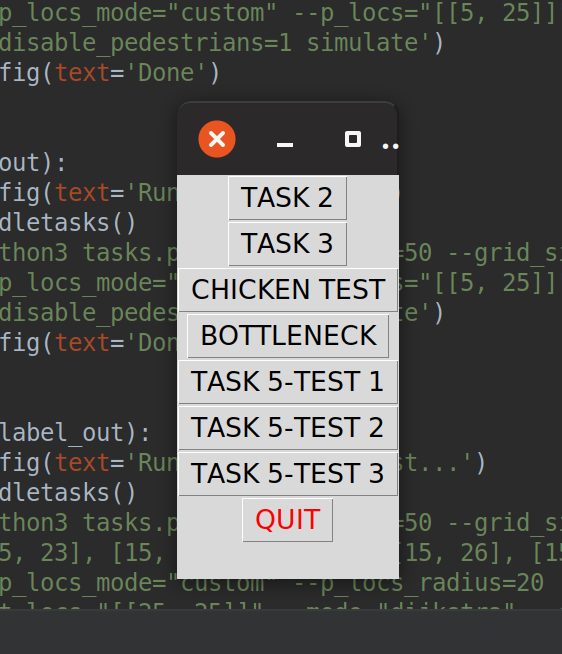
\includegraphics[width=0.5\textwidth]{pictures/gui.png}
    \caption{The simple GUI for running different tasks/scenarios}
    \label{fig:gui}
\end{figure}

\end{task}
\begin{task}{2, First step of a single pedestrian}
The task is to "define a scenario with 50 by 50 cells (2500 in total), a single pedestrian at position (5,25) and a target 20 cells away from them at (25,25)." The pedestrian is supposed to walk in 25 steps to the target and waits there. We set up the scenario successfully. (see Fig. \ref{fig:start_2})\\
\begin{figure}[H]
    \centering
    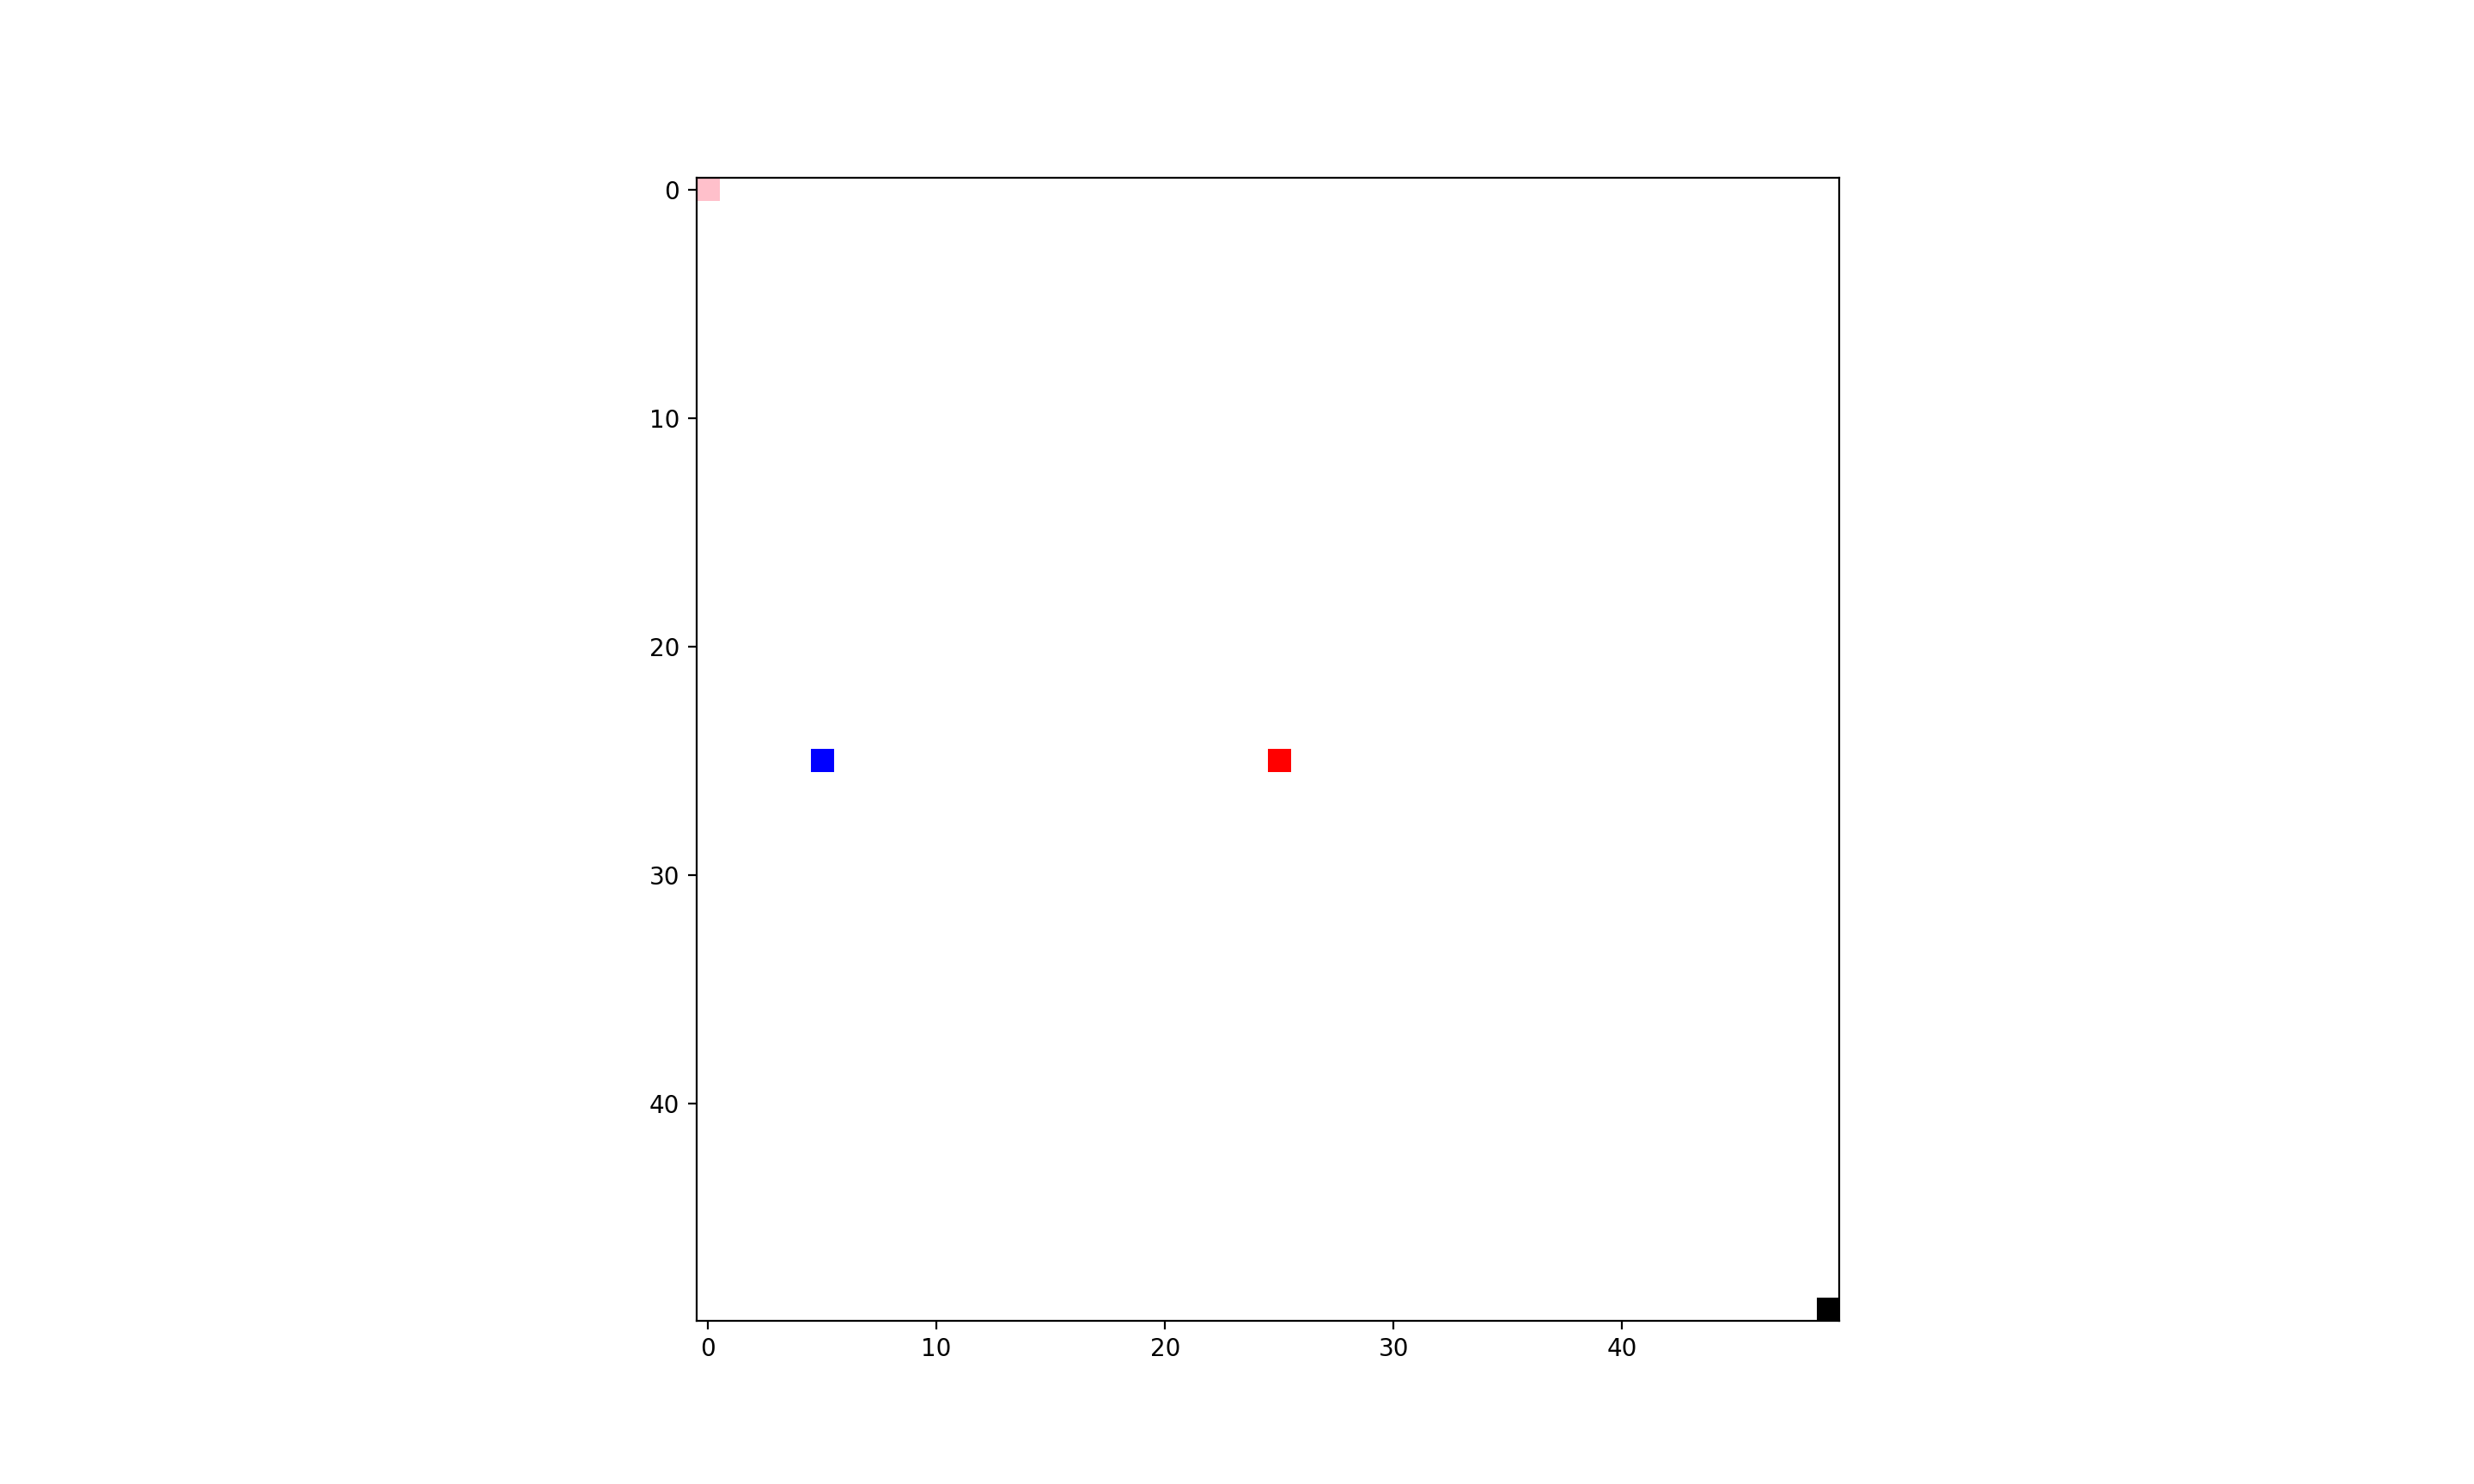
\includegraphics[width=0.85\textwidth]{pictures/2_Start.png}
    \caption{Start scenario of task 2}
    \label{fig:start_2}
\end{figure}
The pedestrian arrives in our scenario successfully at the target. The counter starts counting at zero, therefore the counter shows 24 steps at the end. The successful arrival after 25 steps can be seen in Figure \ref{fig:end_2}. The pedestrian is marked in blue, while the target is colored red. We implemented the path the pedestrian takes in grey, so that it is possible to see which path the pedestrian took. The cellular automaton uses the Dijkstra algorithm to compute the best path from the pedestrian to the target.
\begin{figure}[H]
    \centering
    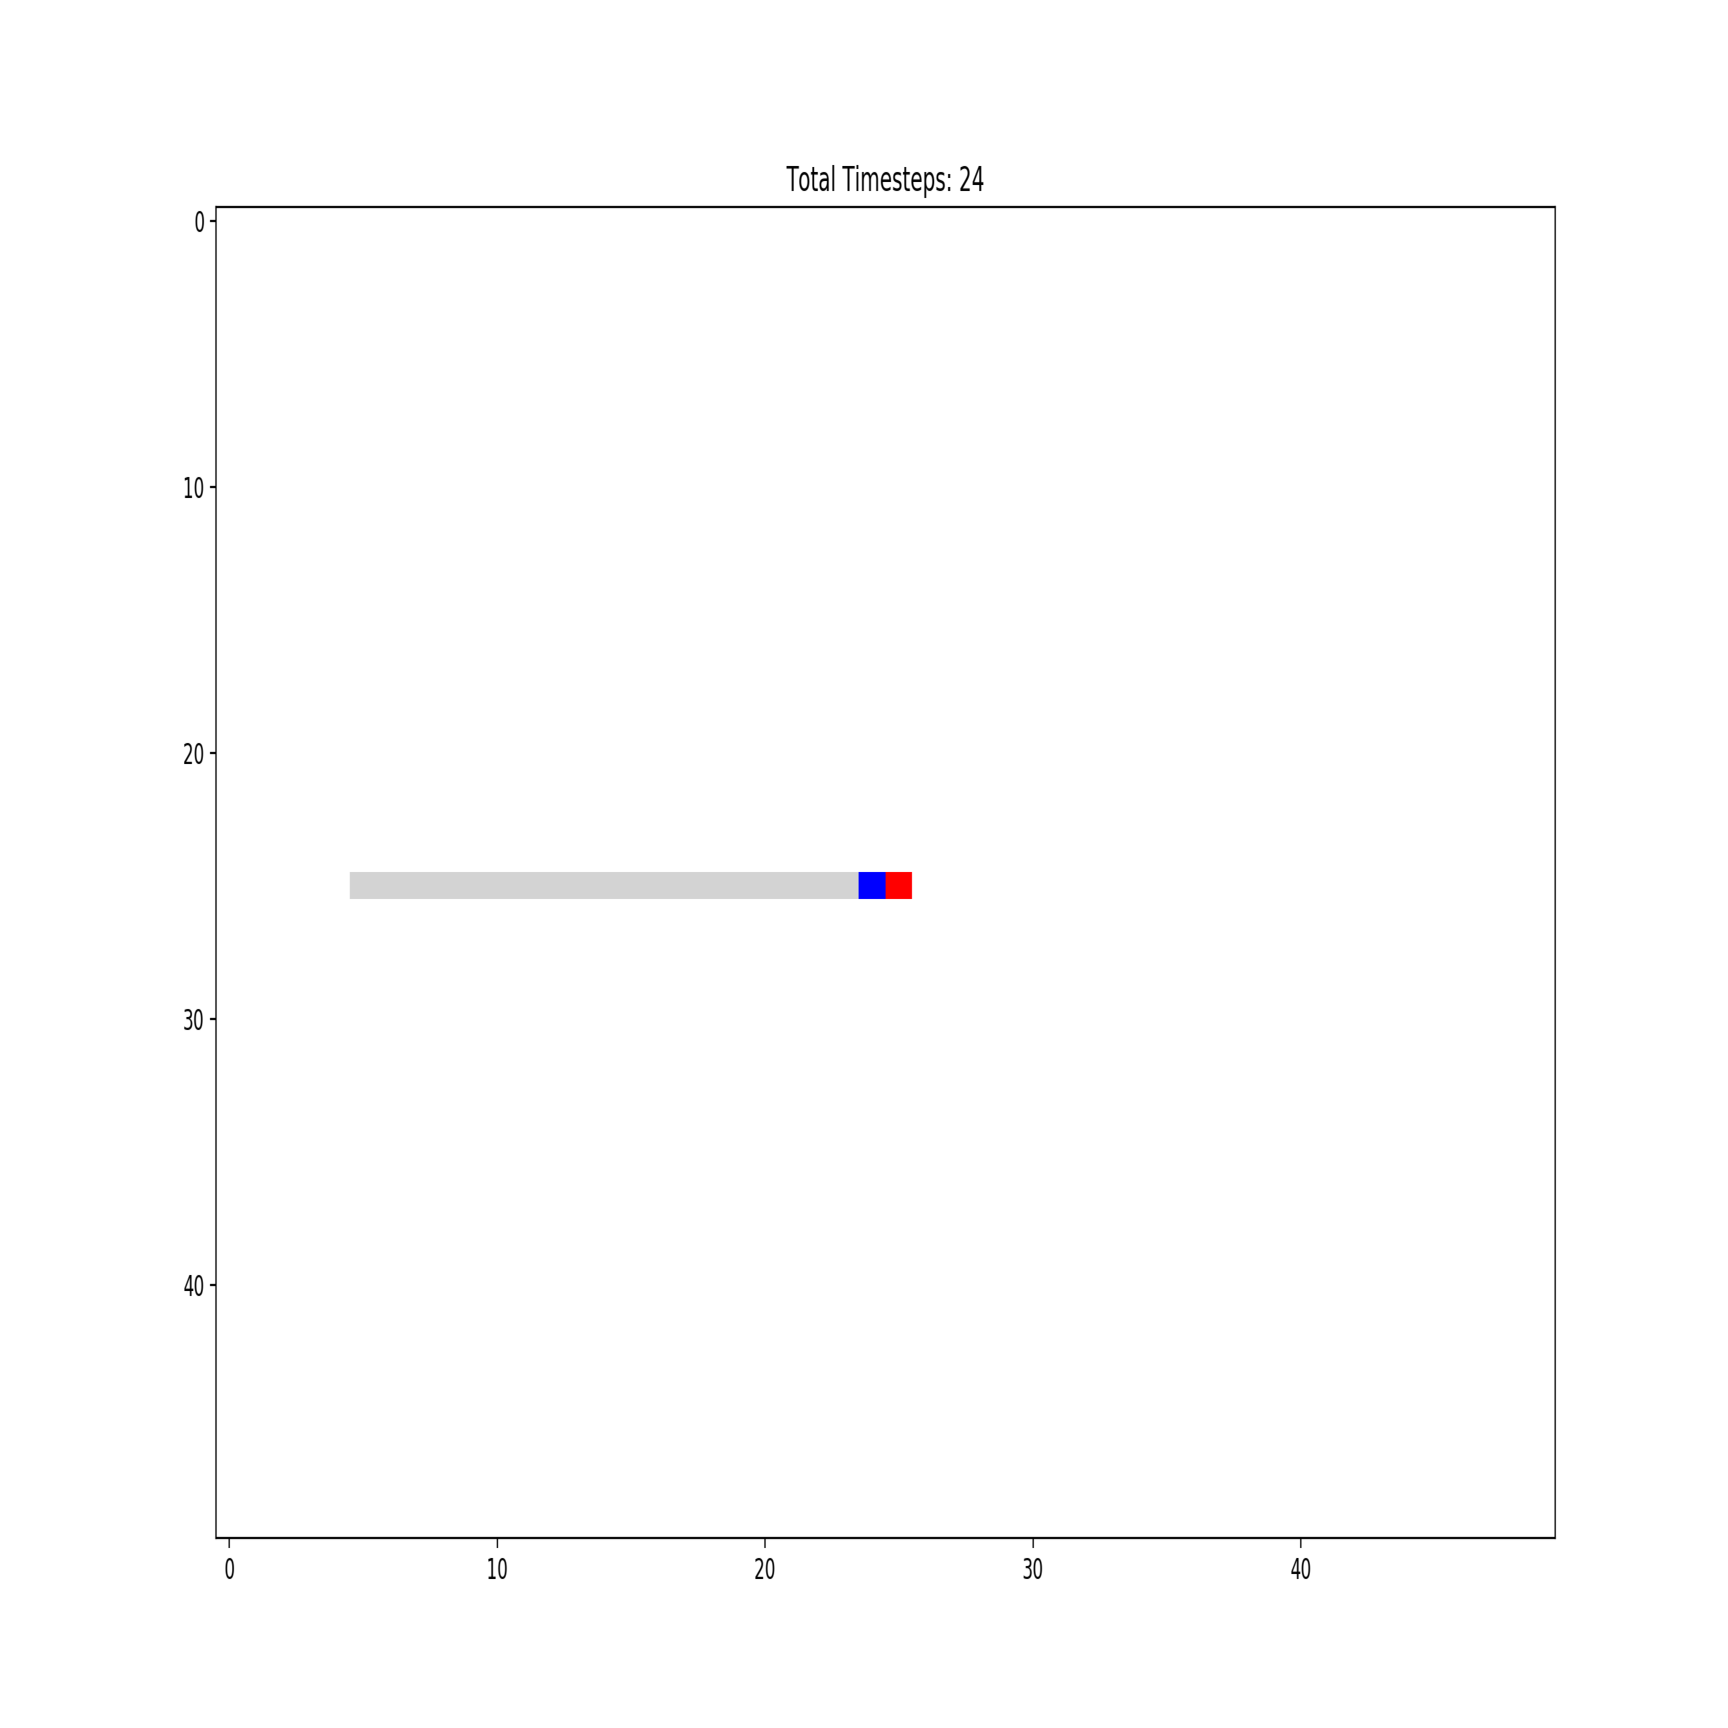
\includegraphics[width=0.52\textwidth]{pictures/End.png}
    \caption{Pedestrian arrived at target successfully and waits}
    \label{fig:end_2}
\end{figure}
\end{task}
\begin{task}{3, Interaction of pedestrians}
We use the previous defined scenario with 50 by 50 cells and a target at position (25,25). In this scenario five pedestrians are inserted in a circle with radius 20 around the target. The starting scenario can be seen in Figure \ref{fig:start_3}, where the pedestrians are marked in blue, while the target is colored in red.
In order to avoid pedestrian collision, for each pedestrian we add a cost for moving to a neighboring tile. For a pedestrian i, this cost is defined by the following formula: \\

\begin{center}
$P_{ik} = \sum_{j}^{N} \frac{1.5}{r_{kj} + \epsilon }$
\end{center}


where $P_{ik}$ is the total pedestrians avoidance cost for pedestrian i upon moving to the neighboring cell k, N is the total number of pedestrians, $r_{kj}$ is the euclidean distance of the cell k to pedestrian j and $\epsilon$ is a very small constant to avoid division by zero. 

\begin{figure}[H]
    \centering
    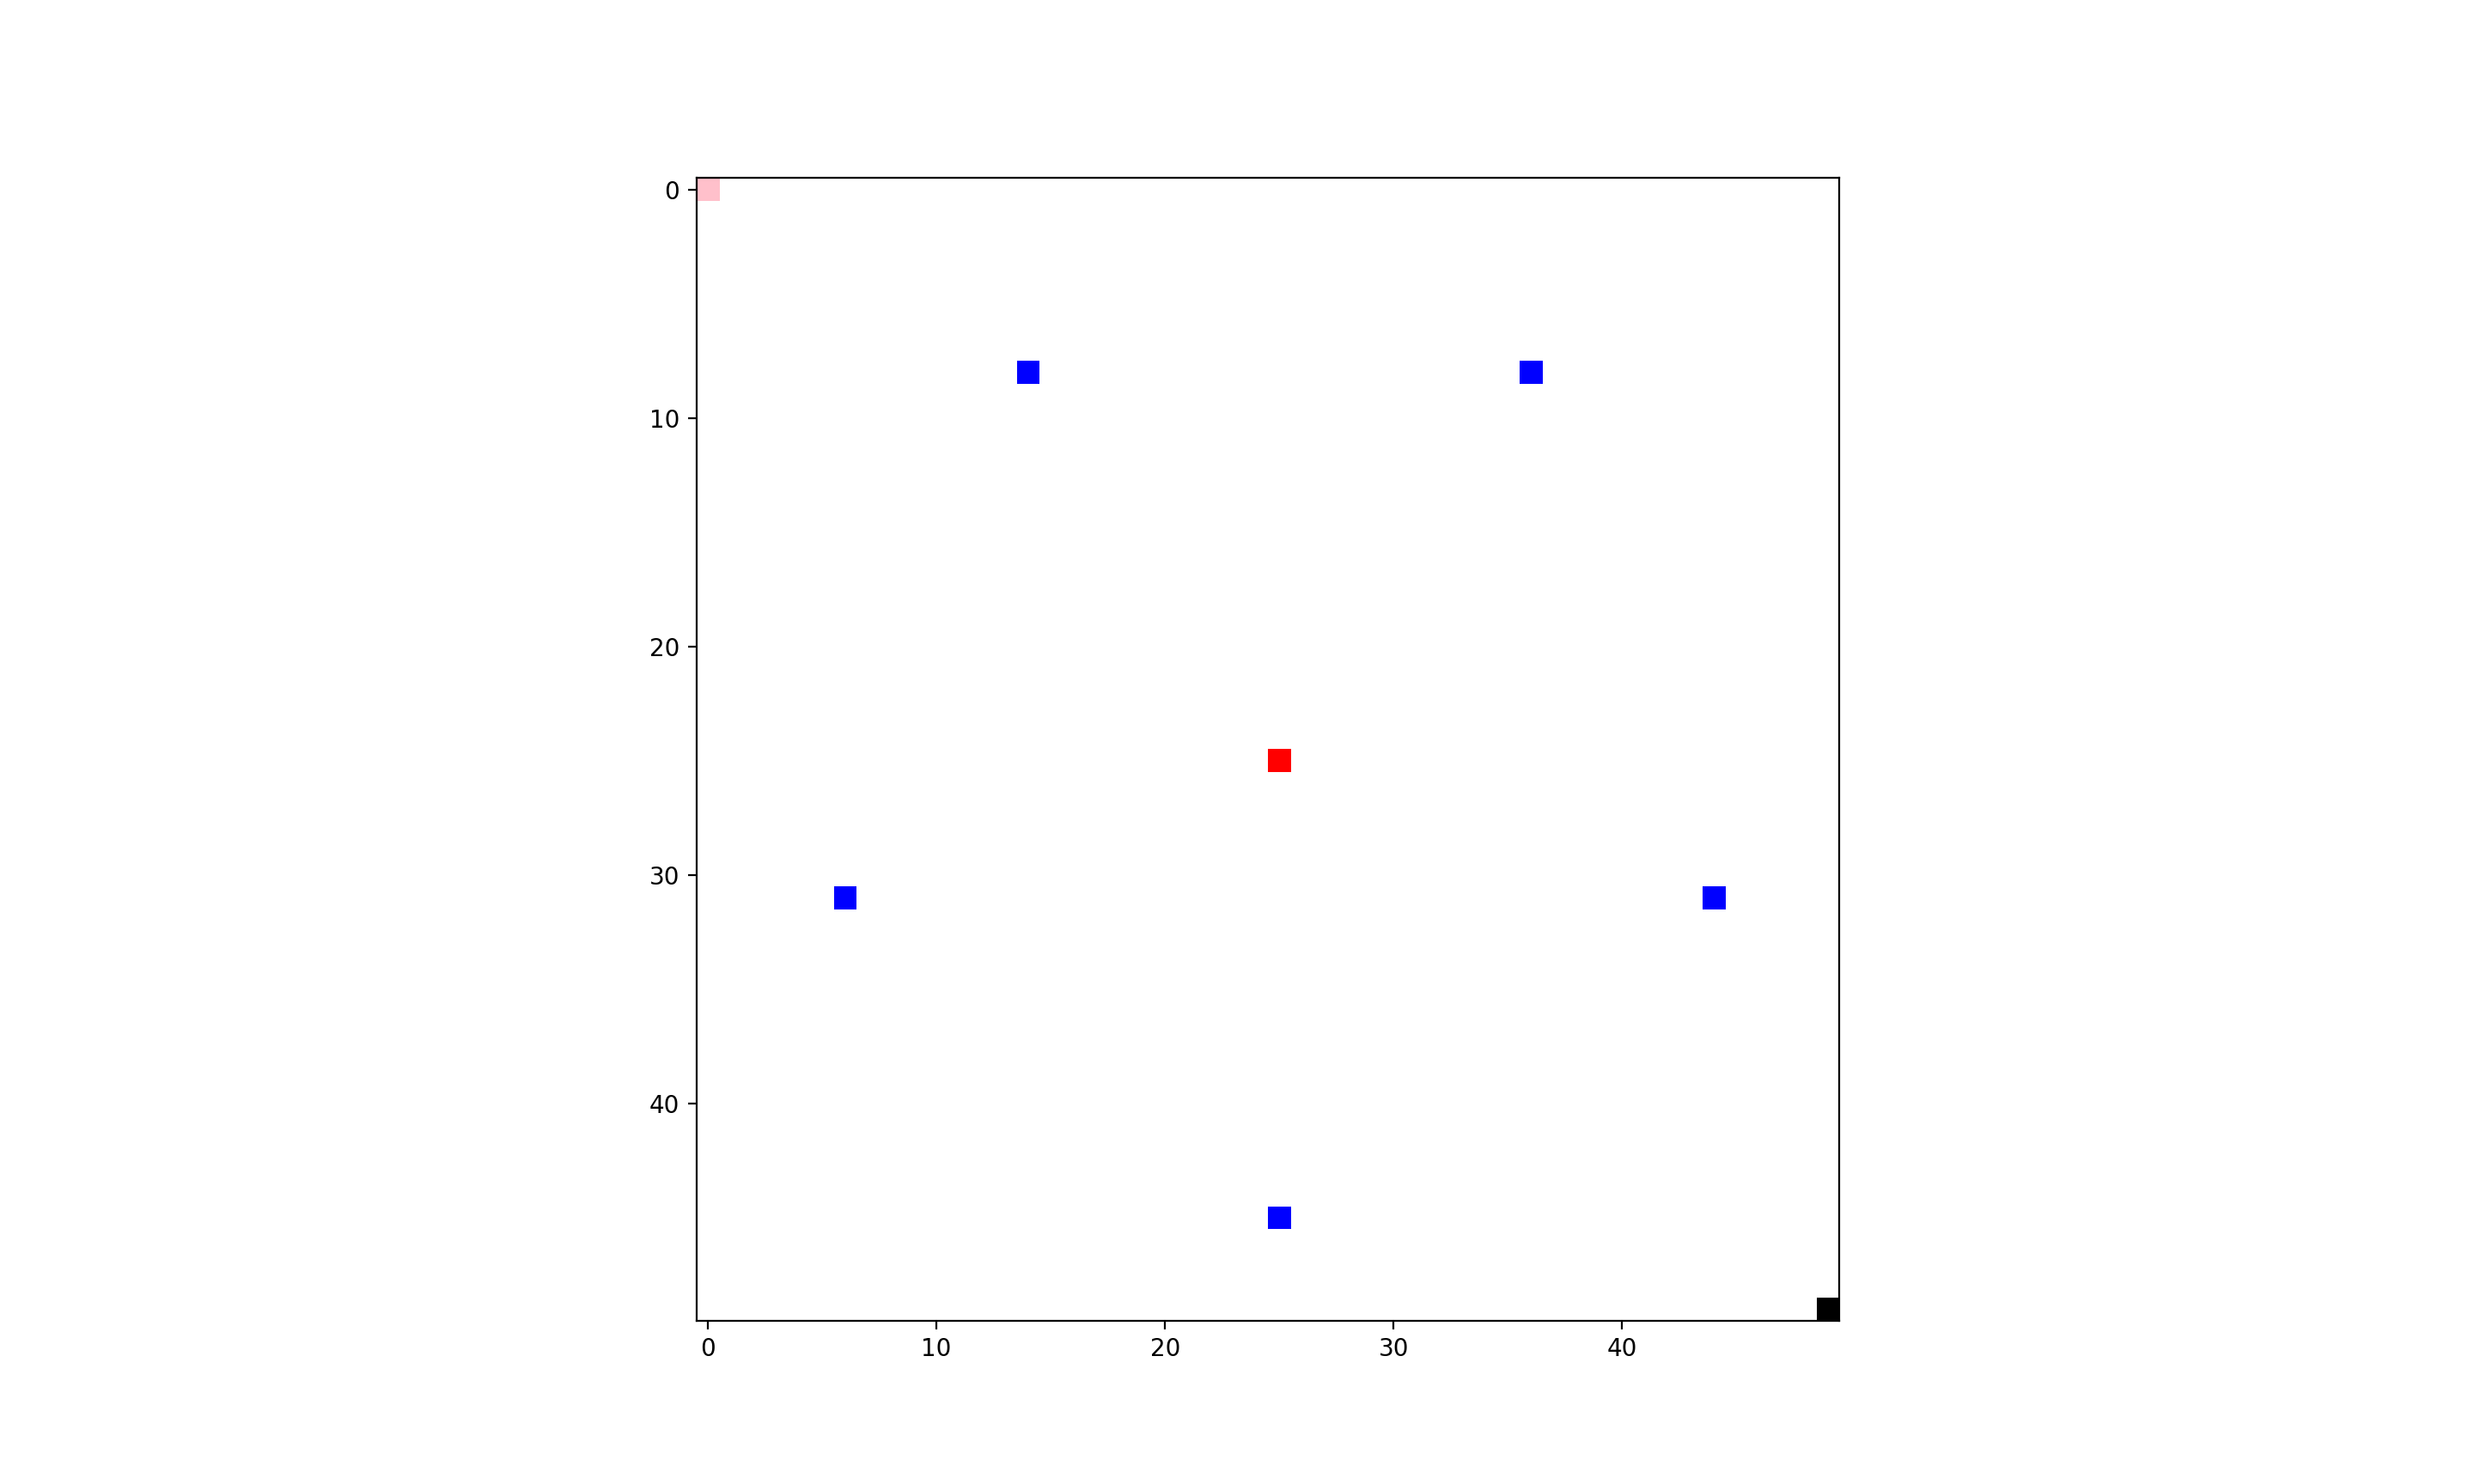
\includegraphics[width=0.85\textwidth]{pictures/Task3_start.png}
    \caption{Setup of Task 3}
    \label{fig:start_3}
\end{figure}
We use the Dijkstra algorithm to find the shortest path from the pedestrians to the target. The paths of all pedestrians are colored in grey. The target has only four sides where pedestrians can reach it. Consequently the first four pedestrians reach the target directly, while the last pedestrian can only queue behind another pedestrian, since the way to the target is already blocked from every side. This can be seen in Figure \ref{fig:3_end}.
\begin{figure}[H]
    \centering
    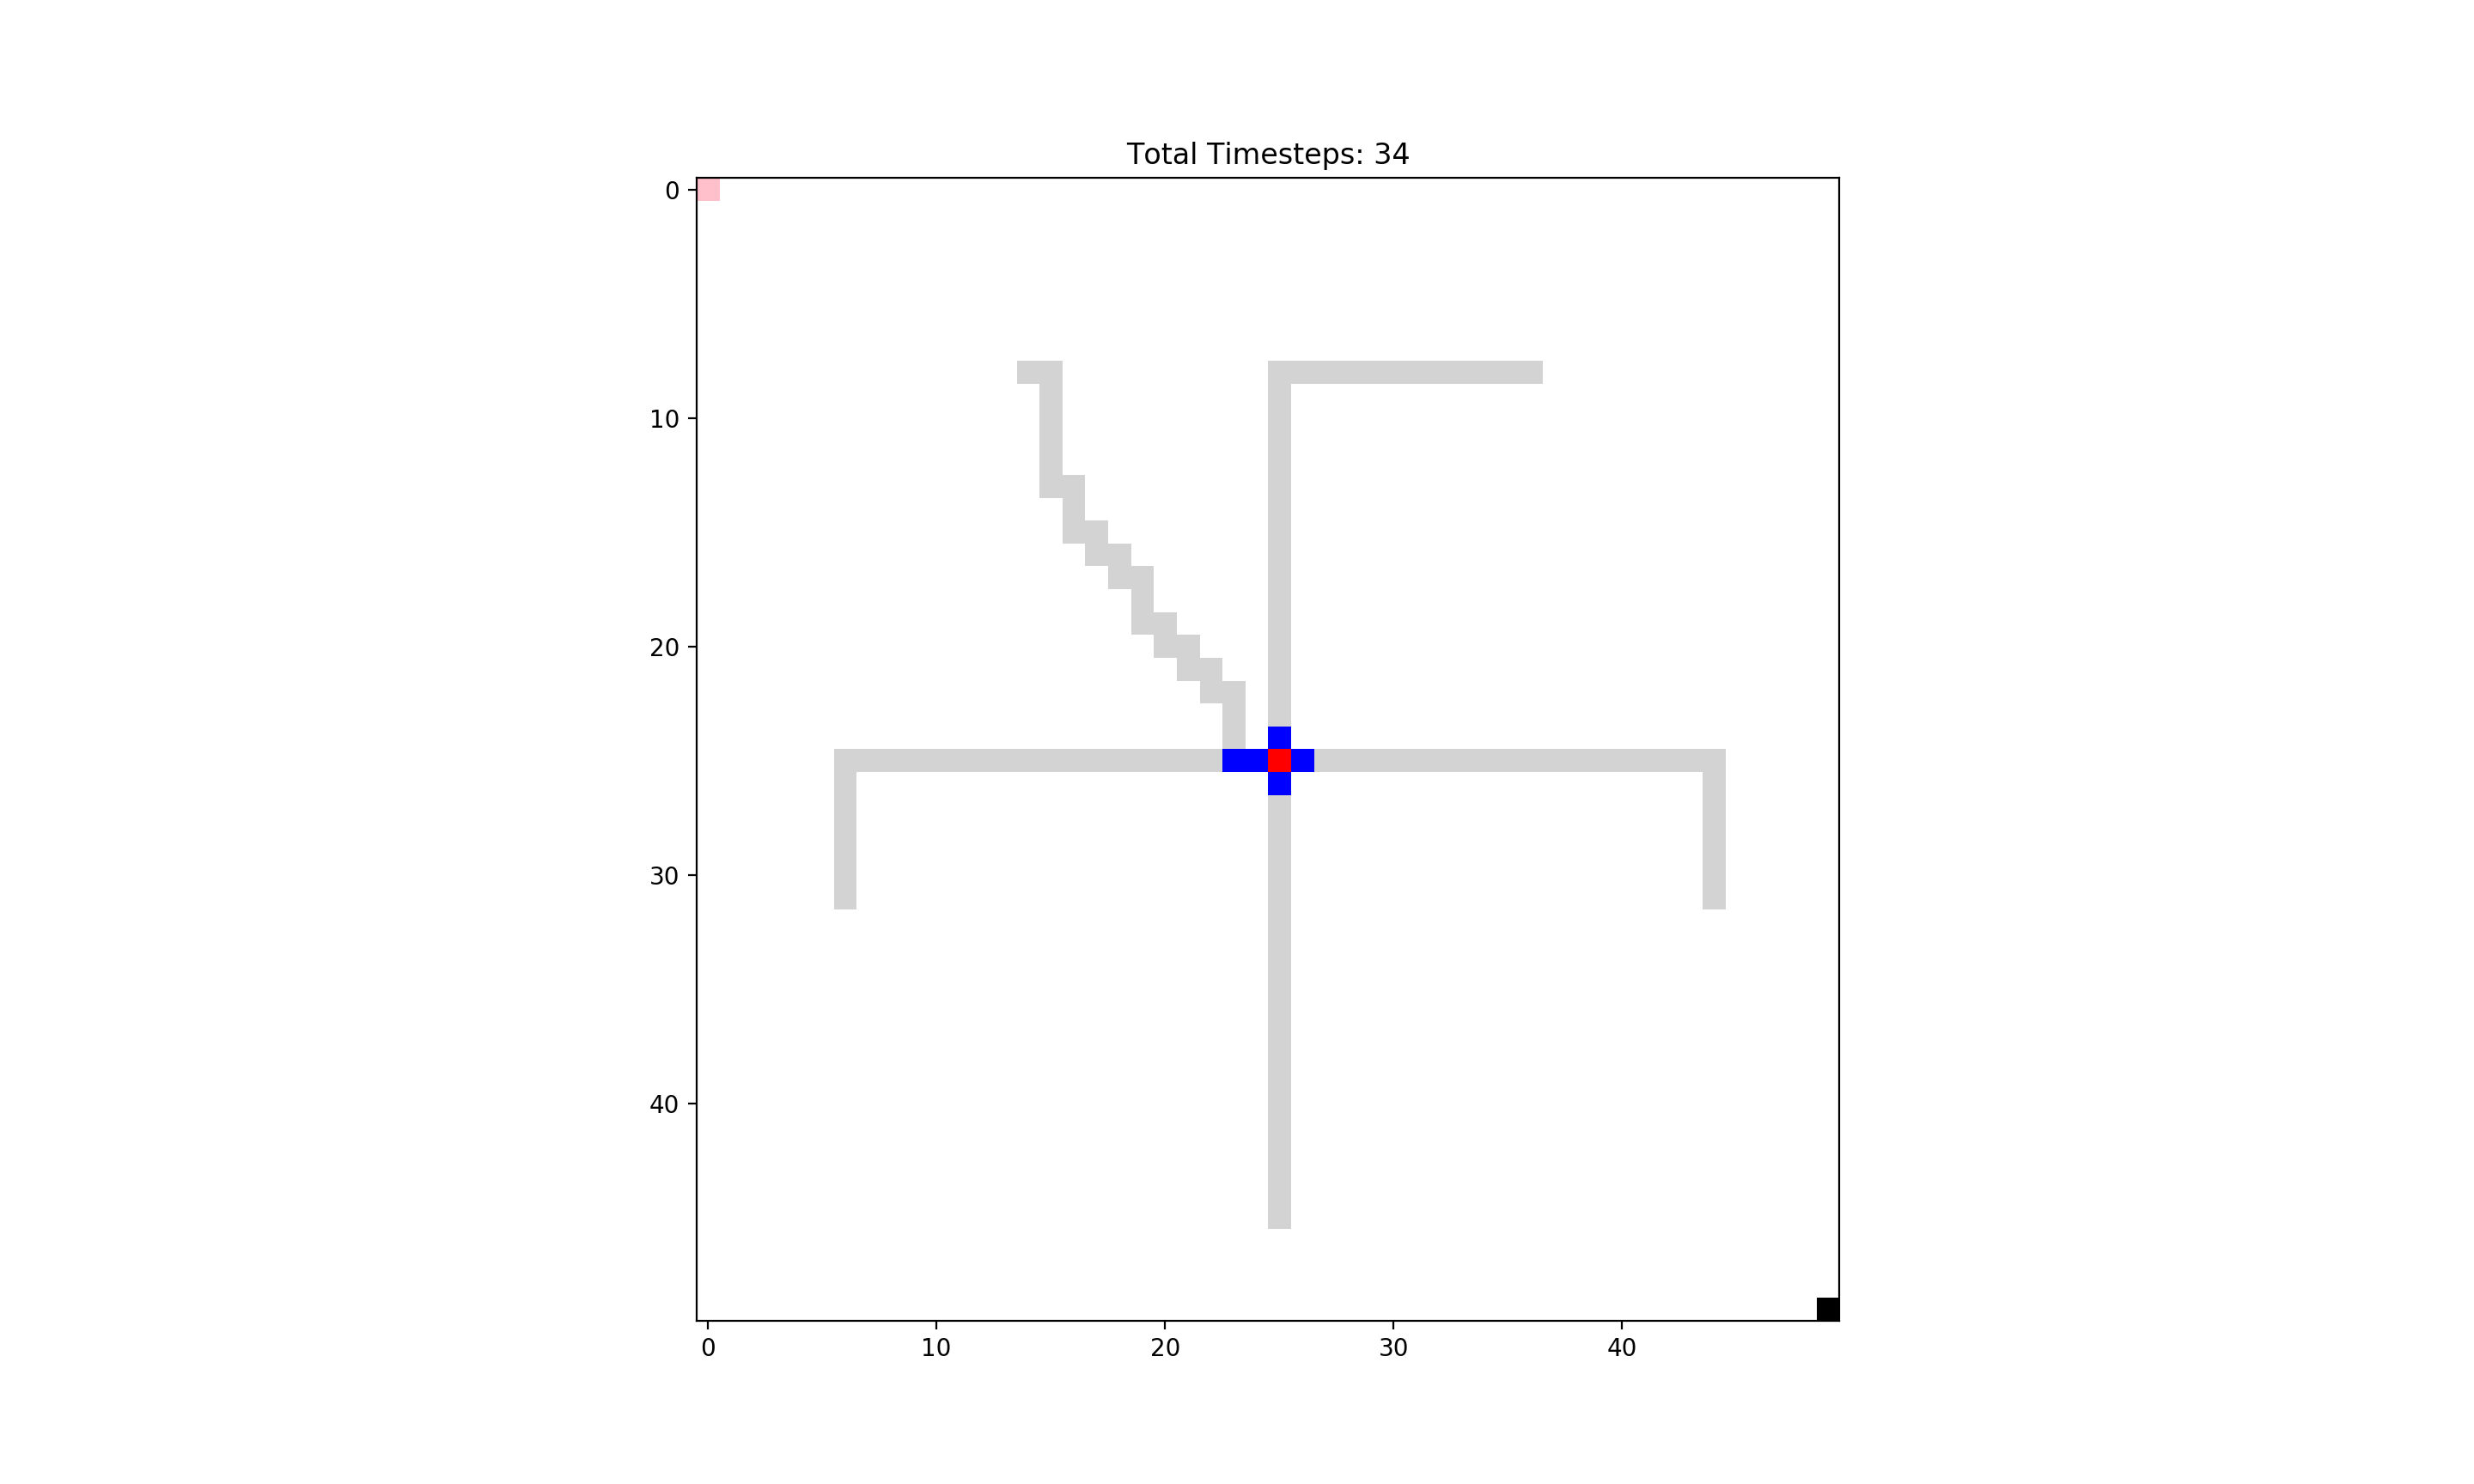
\includegraphics[width=0.85\textwidth]{pictures/Task3_end.png}
    \caption{First pedestrian arrives after 9 steps}
    \label{fig:3_end}
\end{figure}
\end{task}
\newpage
\begin{task}{4, Obstacle avoidance}
As in the case of pedestrian avoidance, for obstacle avoidance a cost is added to the total cost of moving to each neighboring cell for a pedestrian. The cost can be defined by the following formula:

\begin{center}
$O_{ik} = \sum_{j}^{M} \frac{r_{max}}{r_{kj} + \epsilon }$
\end{center}
where $O_{ik}$ is the total obstacle avoidance cost for pedestrian i upon moving to the neighboring cell k, M is the total number of obstacles, $r_{kj}$ is the euclidean distance of the cell k to obstacle j, $r_{max} = max(grid\_size\_x, grid\_size\_y)$ and $\epsilon$ is a very small constant to avoid division by zero.\\ 
The pedestrians managed to avoid the obstacle in the chicken test, and each other in the bottleneck test using Dijkstra’s algorithm.
As seen in Figure \ref{fig:obst_start}, the target is on the same y axis as the pedestrian. If the obstacles were to be ignored, the shortest path would have been to go straight down, but the pedestrian would have gotten stuck. \\

\begin{figure}[H]
    \centering
    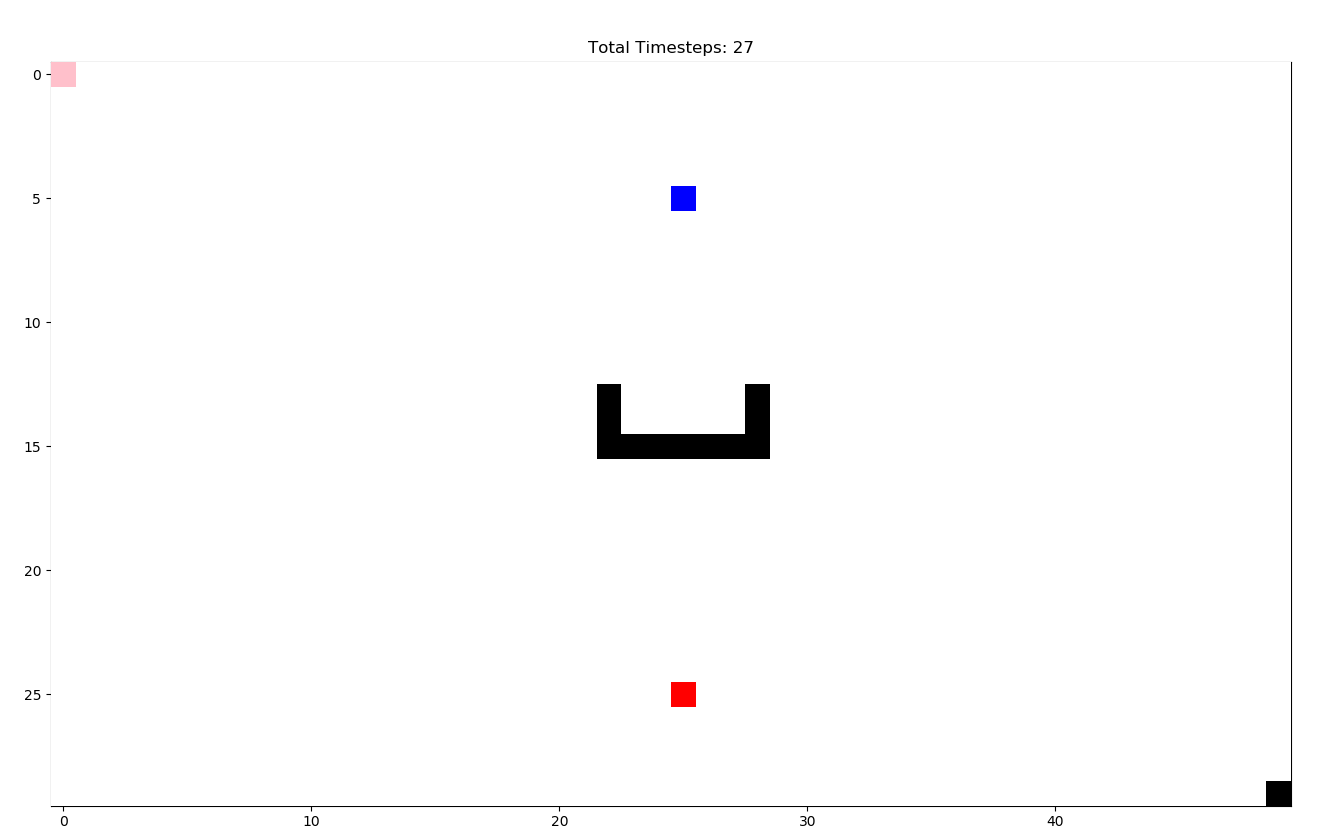
\includegraphics[width=0.65\textwidth]{pictures/start_task4_obst.PNG}
    \caption{Initialization of the chicken test.}
    \label{fig:obst_start}
\end{figure}
However, as seen in Figure \ref{fig:obst_end}, the pedestrian walks around the obstacle and reaches the target with the shortest path possible, since Dijkstra’s algorithm guarantees completeness and optimality. \\
\begin{figure}[H]
    \centering
    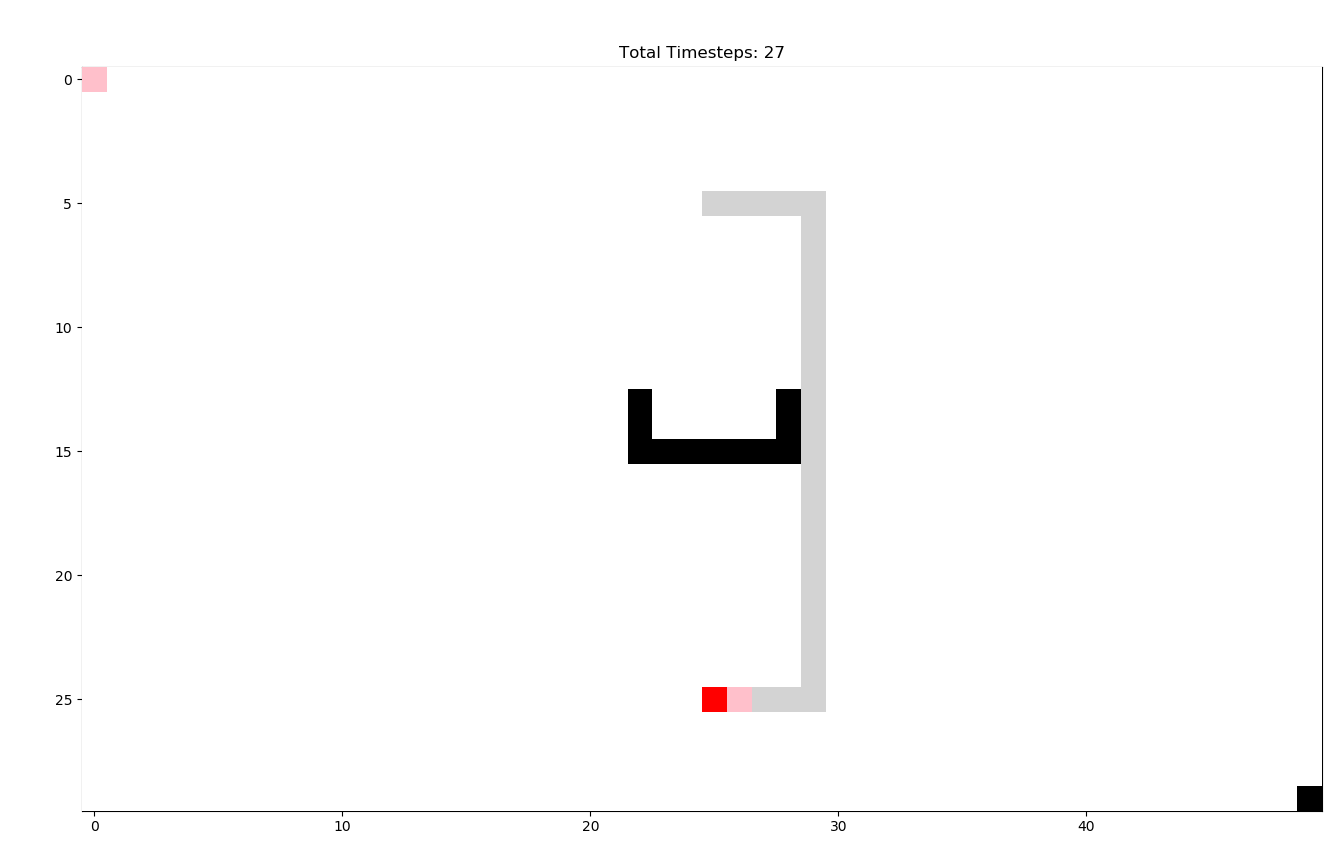
\includegraphics[width=0.65\textwidth]{pictures/end_task4_obst.PNG}
    \caption{The pedestrian successfully avoids the concave obstacle.}
    \label{fig:obst_end}
\end{figure}
Moreover, obstacle avoidance has been tested with a case of possible congestion as well. As seen in Figure \ref{fig:cong_start}, there are 3 pedestrians next to each other in an enclosed area with a 1 block wide exit. 
\begin{figure}[H]
    \centering
    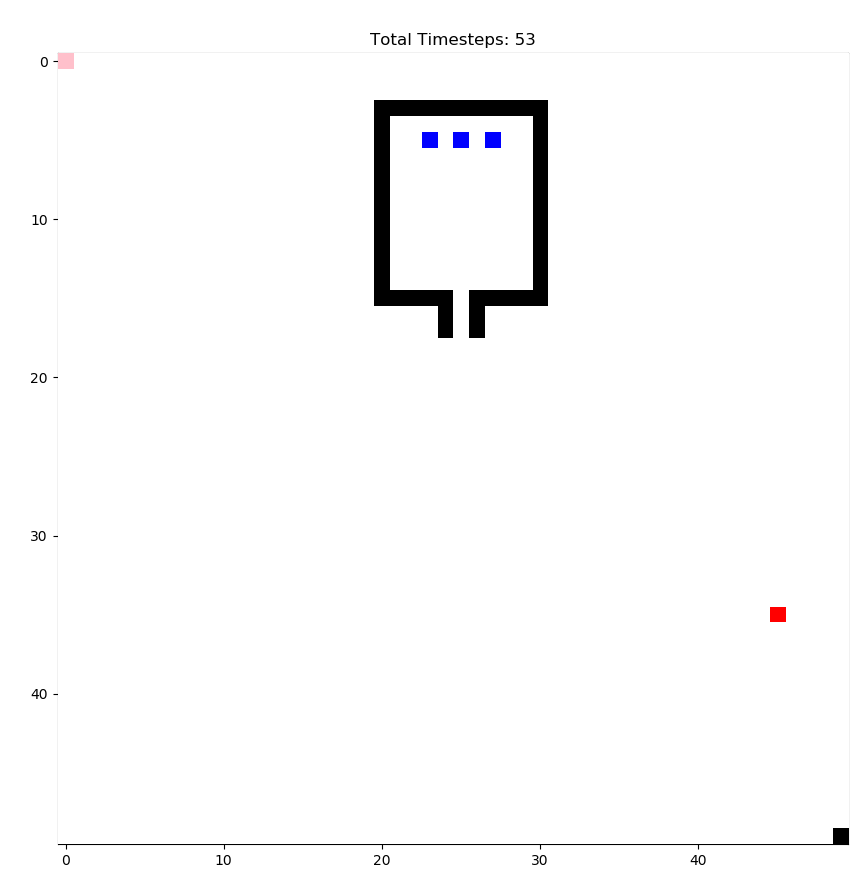
\includegraphics[width=0.5\textwidth]{pictures/start_task4_cong.PNG}
    \caption{Initialisation of the congestion test.}
    \label{fig:cong_start}
\end{figure}
As they reach the tight passage, pedestrians avoid hitting each other and wait for the other pedestrians to go through (see Figure \ref{fig:cong_mid}). 
\begin{figure}[H]
    \centering
    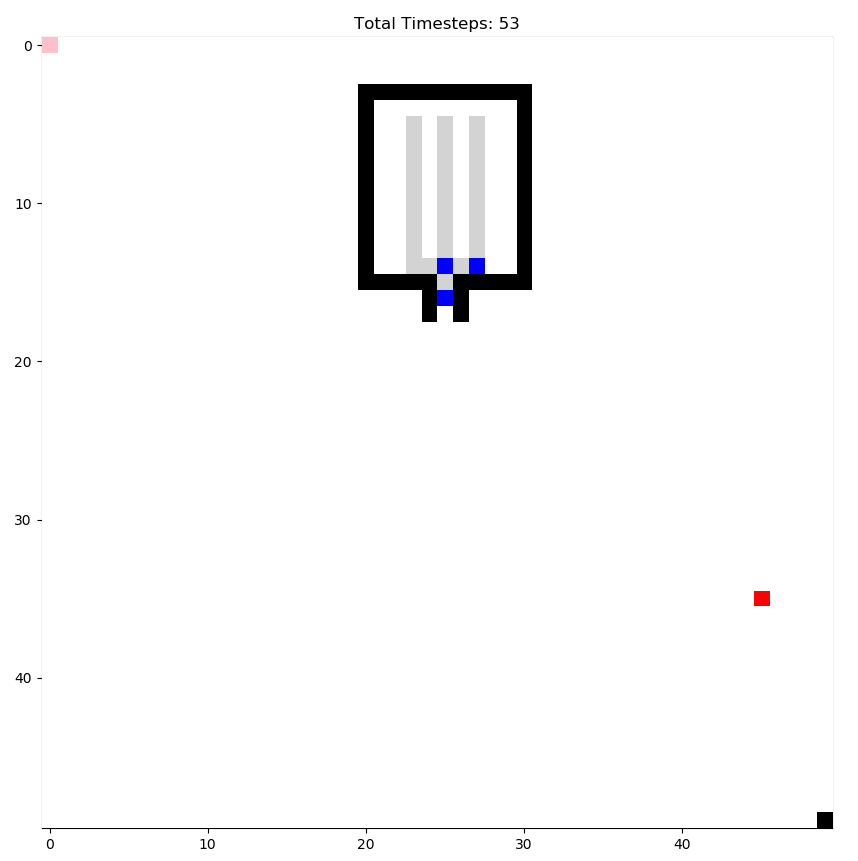
\includegraphics[width=0.5\textwidth]{pictures/mid_task4_cong.PNG}
    \caption{The middle pedestrian goes through first. The right one goes 1 block right and waits for the left one to go through.}
    \label{fig:cong_mid}
\end{figure}
Every pedestrian reaches the target successfully and they even take different optimal paths as seen in Figure \ref{fig:cong_end}. \\
\begin{figure}[H]
    \centering
    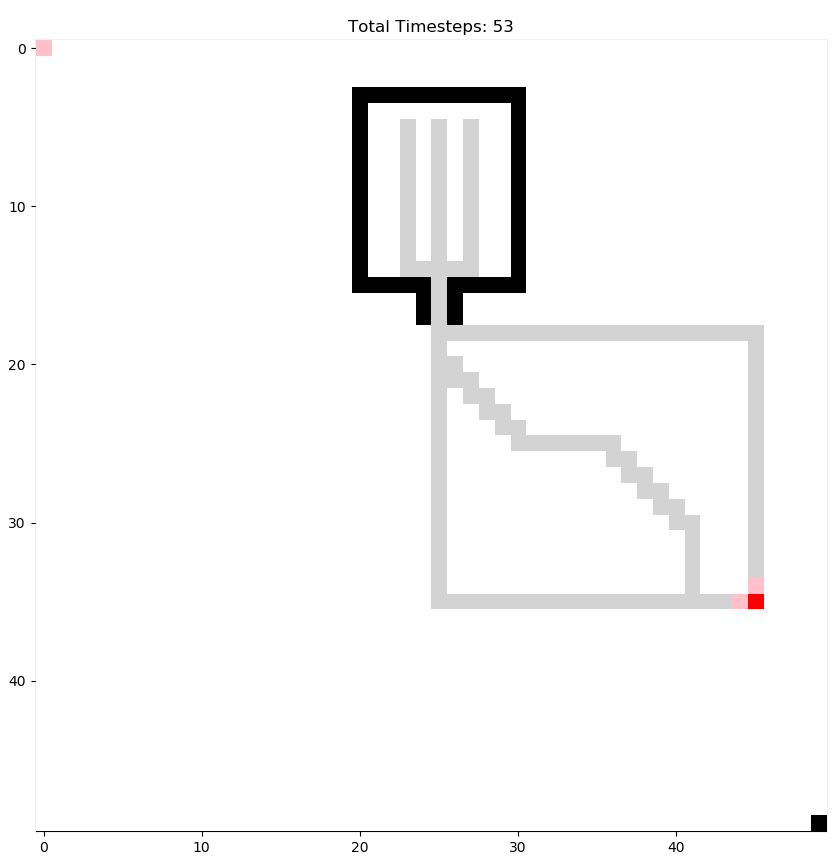
\includegraphics[width=0.5\textwidth]{pictures/end_task4_cong.PNG}
    \caption{The pedestrians successfully avoid each other at the tight passage and reach the target.}
    \label{fig:cong_end}
\end{figure}
If obstacle avoidance were not implemented, only the pedestrian in the middle could have got out and the other two would be stuck as illustrated in Figure \ref{fig:cong_stuck}. \\
\begin{figure}[H]
    \centering
    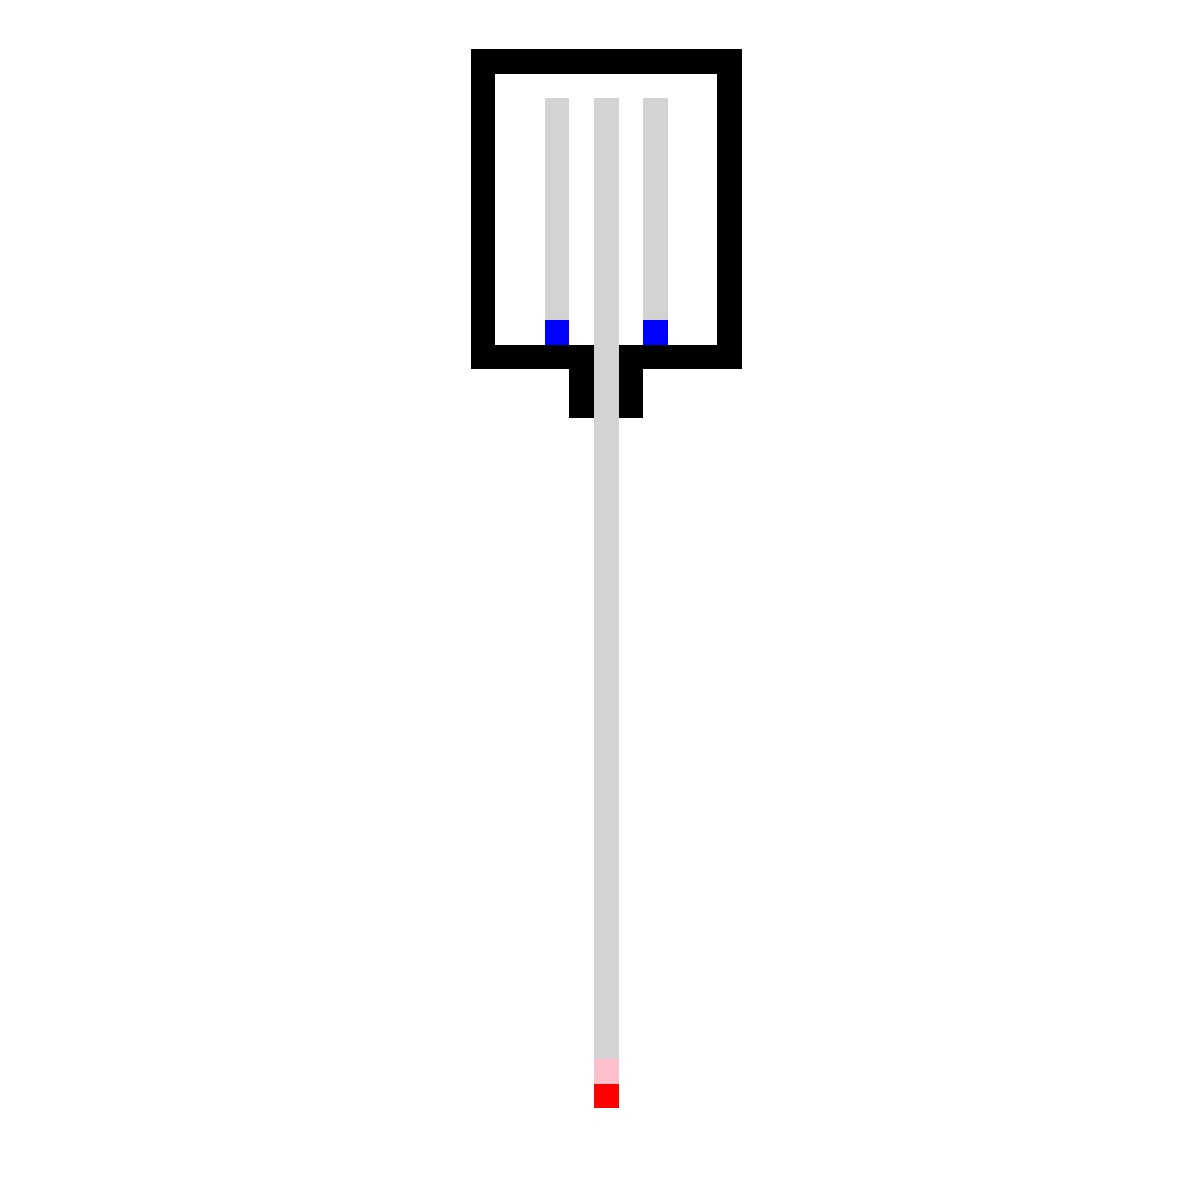
\includegraphics[width=0.5\textwidth]{pictures/task4_cong_stuck.jpeg}
    \caption{The middle pedestrian manages to get out whilst the others just get stuck.}
    \label{fig:cong_stuck}
\end{figure}
\end{task}
\newpage
\begin{task}{5, Tests}
\begin{enumerate}
\item[TEST1:] The RiMEA scenario 1 (straight line, ignore premovement time)\\
- The first test corresponds to the RiMEA scenario one, where one pedestrian which corresponds to 40 centimeters walks down a floor with a length of 40 meters and a width of 2 meters in between 26 and 34 seconds. The pedestrian has to walk with a speed between 4.5 km/h and 5.1 km/h. \\
- The pedestrian has to be 40 centimeters. The side of one cell is 40 centimeters long, since in our cellular automaton a cell corresponds to a pedestrian. As a consequence of that the floor has a length of 100 cells and a width of 5 cells. The setup can be seen in Figure \ref{fig:setup_test1}.
\begin{figure}[H]
    \centering
    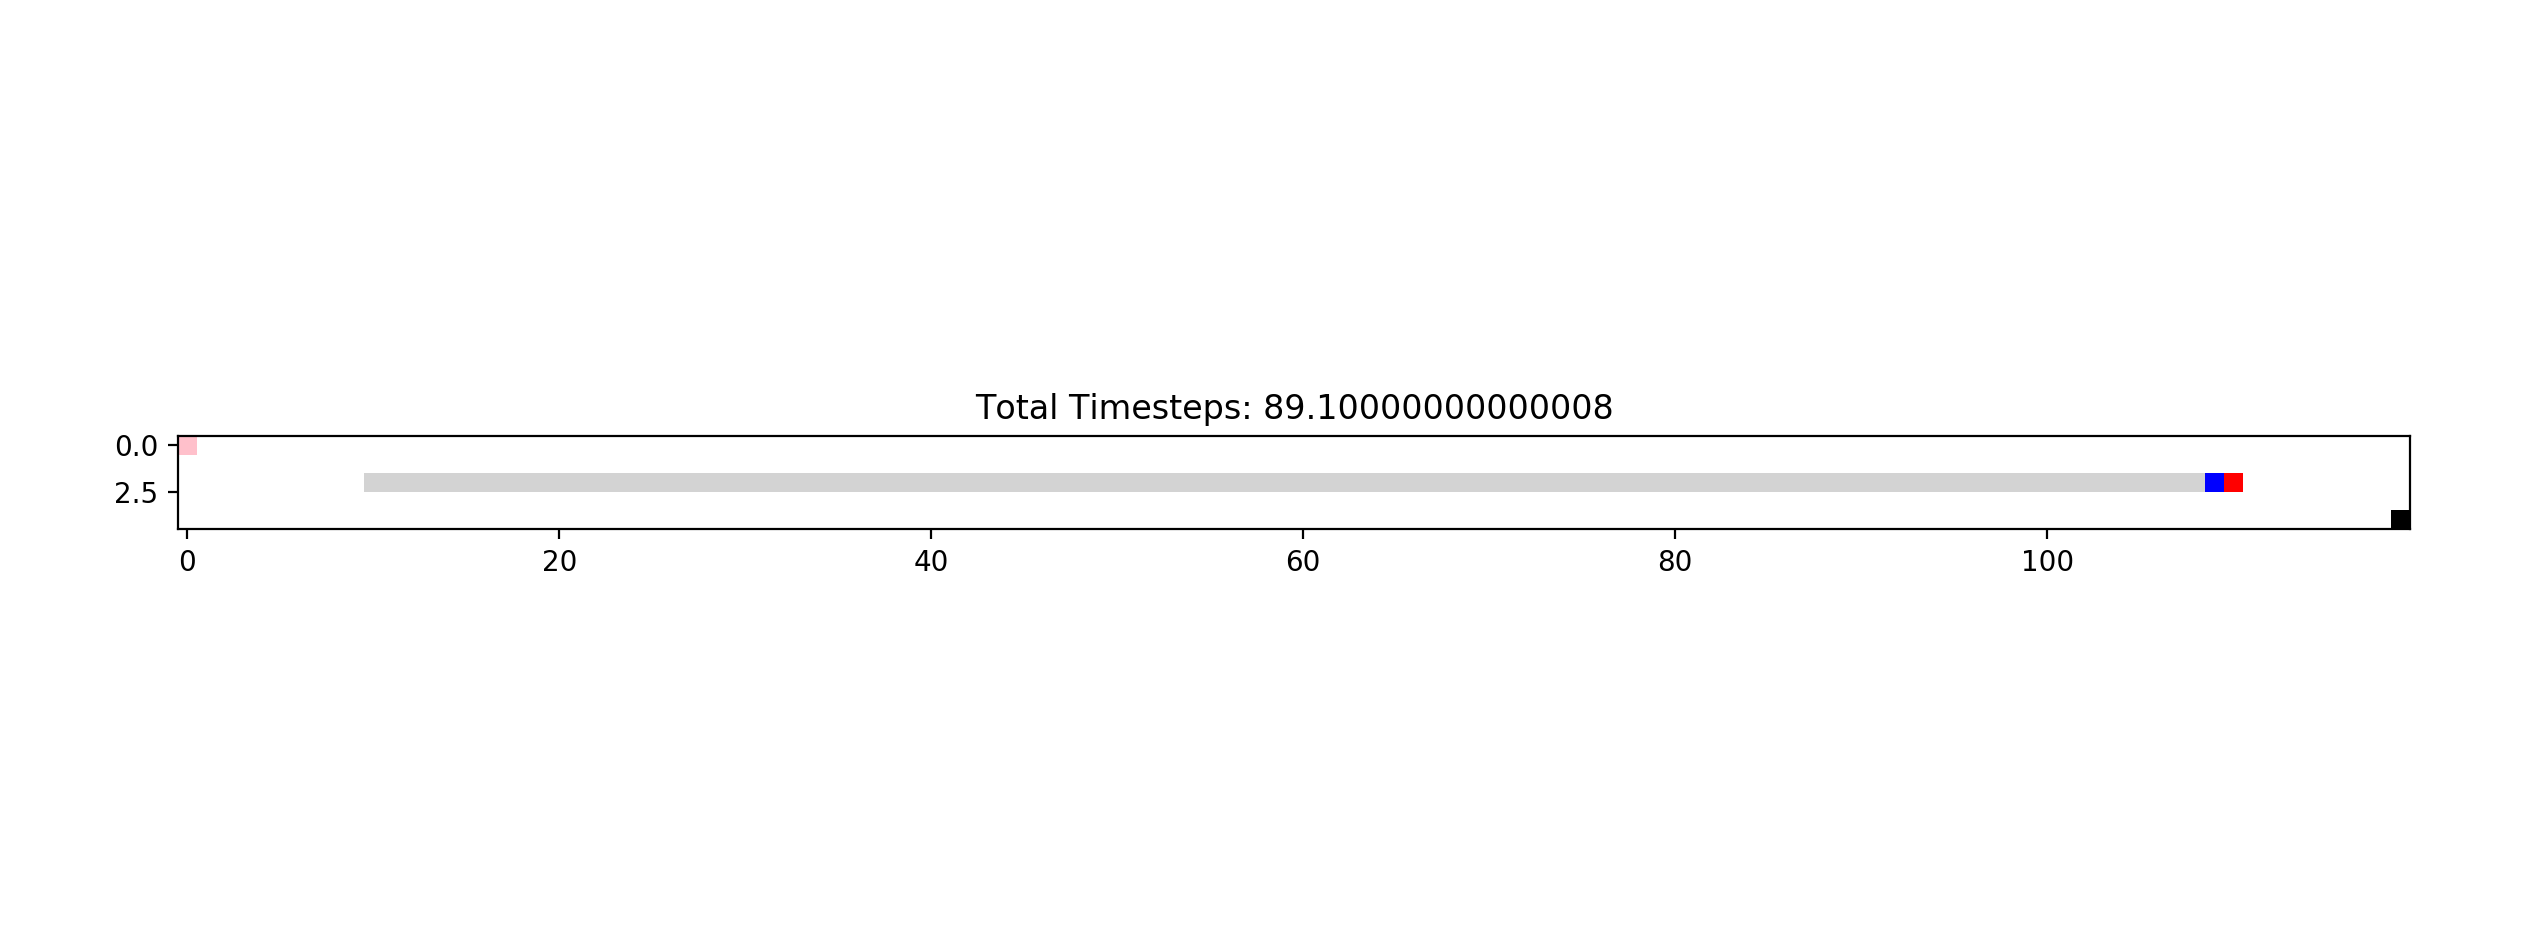
\includegraphics[width=0.8\textwidth]{pictures/Test1start.png}
    \caption{Setup of the RiMEA scenario one}
    \label{fig:setup_test1}
\end{figure}
One timestep in our simulation corresponds to $\frac{1}{3}$ of a second. The pedestrian has a walking speed of 1.33 $\frac{m}{s}$. It arrives after roughly 89 timesteps at the target (see Fig. \ref{fig:result_test1}). Consequently it takes 29,67 seconds for the pedestrian to walk down the floor. This is exactly in the given range of 26 to 34 seconds. So the test is passed successfully \\
- test successful
\begin{figure}[H]
    \centering
    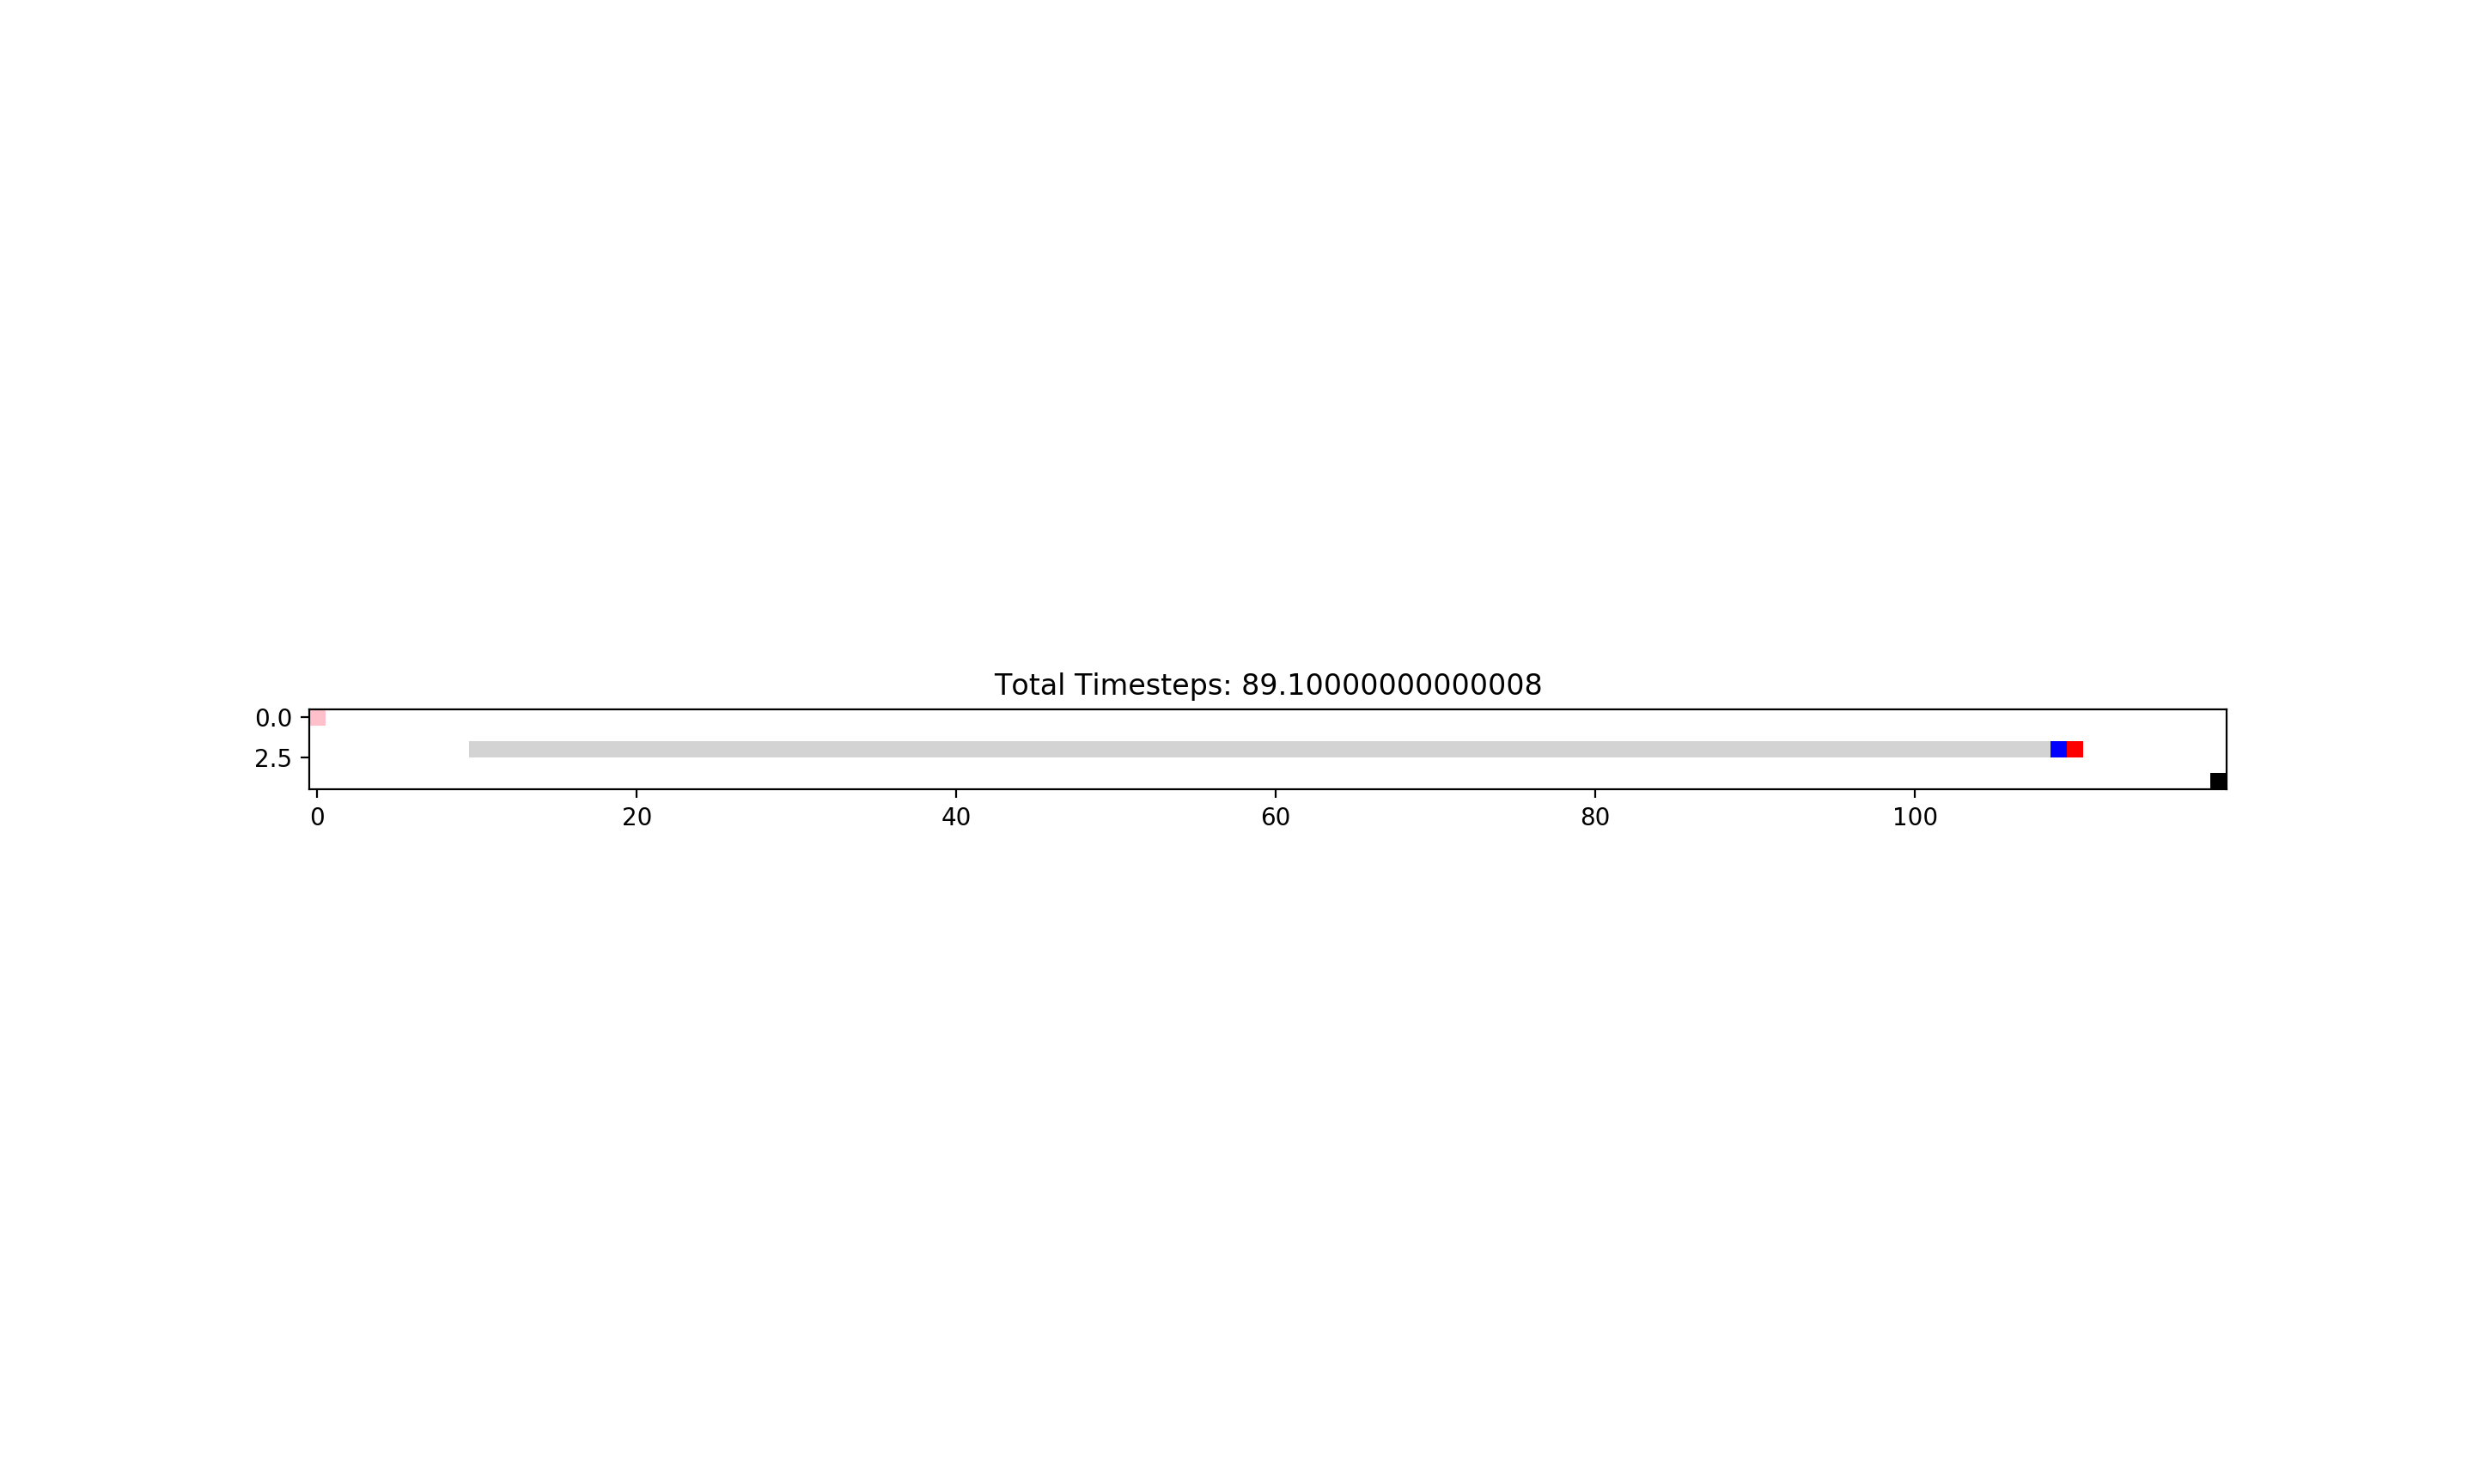
\includegraphics[width=0.9\textwidth]{pictures/test1_end.png}
    \caption{Arrival at the end of the floor after roughly 89 timesteps}
    \label{fig:result_test1}
\end{figure}
\item[TEST2:] RiMEA scenario 4 (fundamental diagram, be careful with periodic boundary conditions).\\
- The second test corresponds to the RiMEA scenario four, where multiple pedestrians uniformly placed with a density value are going from left to right in a 1000 meter long passage with a width of 10 meters. Again, the width of a pedestrian is set 40 centimeters, thus a side of a cell is 40 centimeters long. The pedestrians walk at a speed of 1,2 $\frac{m}{s}$. There are measuring points of area 2 by 2 meters at 450 and 500 meters. The latter is the main measuring point. \\
- A single time step is set as a third of a second. So the pedestrians move 1 cell per time step. The length of the corridor is 2500 blocks and its width is 25 blocks. \\
- At each time step ranging from the 1\textsuperscript{st} to the 180\textsuperscript{th} time step (total of 60 seconds), the number of pedestrians present on the measuring point are added to the sum. After the simulation, the sum is divided by the time passed to get an average number of people per unit time in that area. Then the value is divided by the are of measuring point to get the density in that area. Finally, the density is multiplied by the pedestrian speed to get the flow of the measuring point. As seen in Figure \ref{fig:test2_result}, as the pedestrian density at initialization increases, the flow increases linearly. \\
- test successful - \\
\begin{figure}[H]
    \centering
    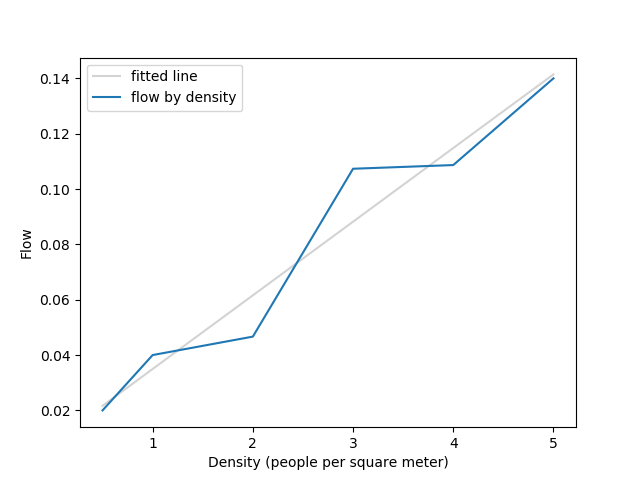
\includegraphics[width=\textwidth]{pictures/test2result.png}
    \caption{The increase of flow per density is linear.}
    \label{fig:test2_result}
\end{figure}
\newpage
\item[TEST3:] RiMEA scenario 6 (movement around a corner).\\
- The third test corresponds to RiMEA scenario 6 which is executed successfully if twenty uniformly distributed people walk around a left corner without passing through any walls. The starting setup can be seen in Figure \ref{fig:corner}.
\begin{figure}[H]
    \centering
    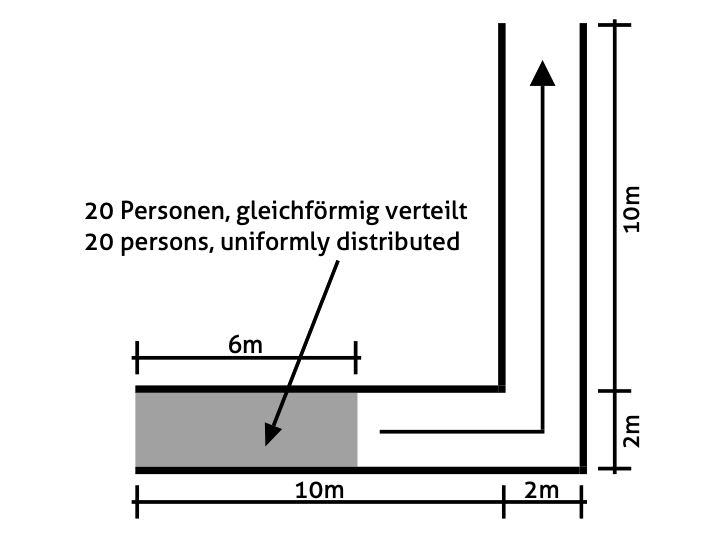
\includegraphics[width=0.5\textwidth]{pictures/corner.png}
    \caption{Setup of RiMEA scenario 6}
    \label{fig:corner}
\end{figure}
Figure \ref{fig:test5_1} shows one setup scenario of our simulation where 20 pedestrians are uniformly distributed before the corner.\\
\begin{figure}[H]
    \centering
    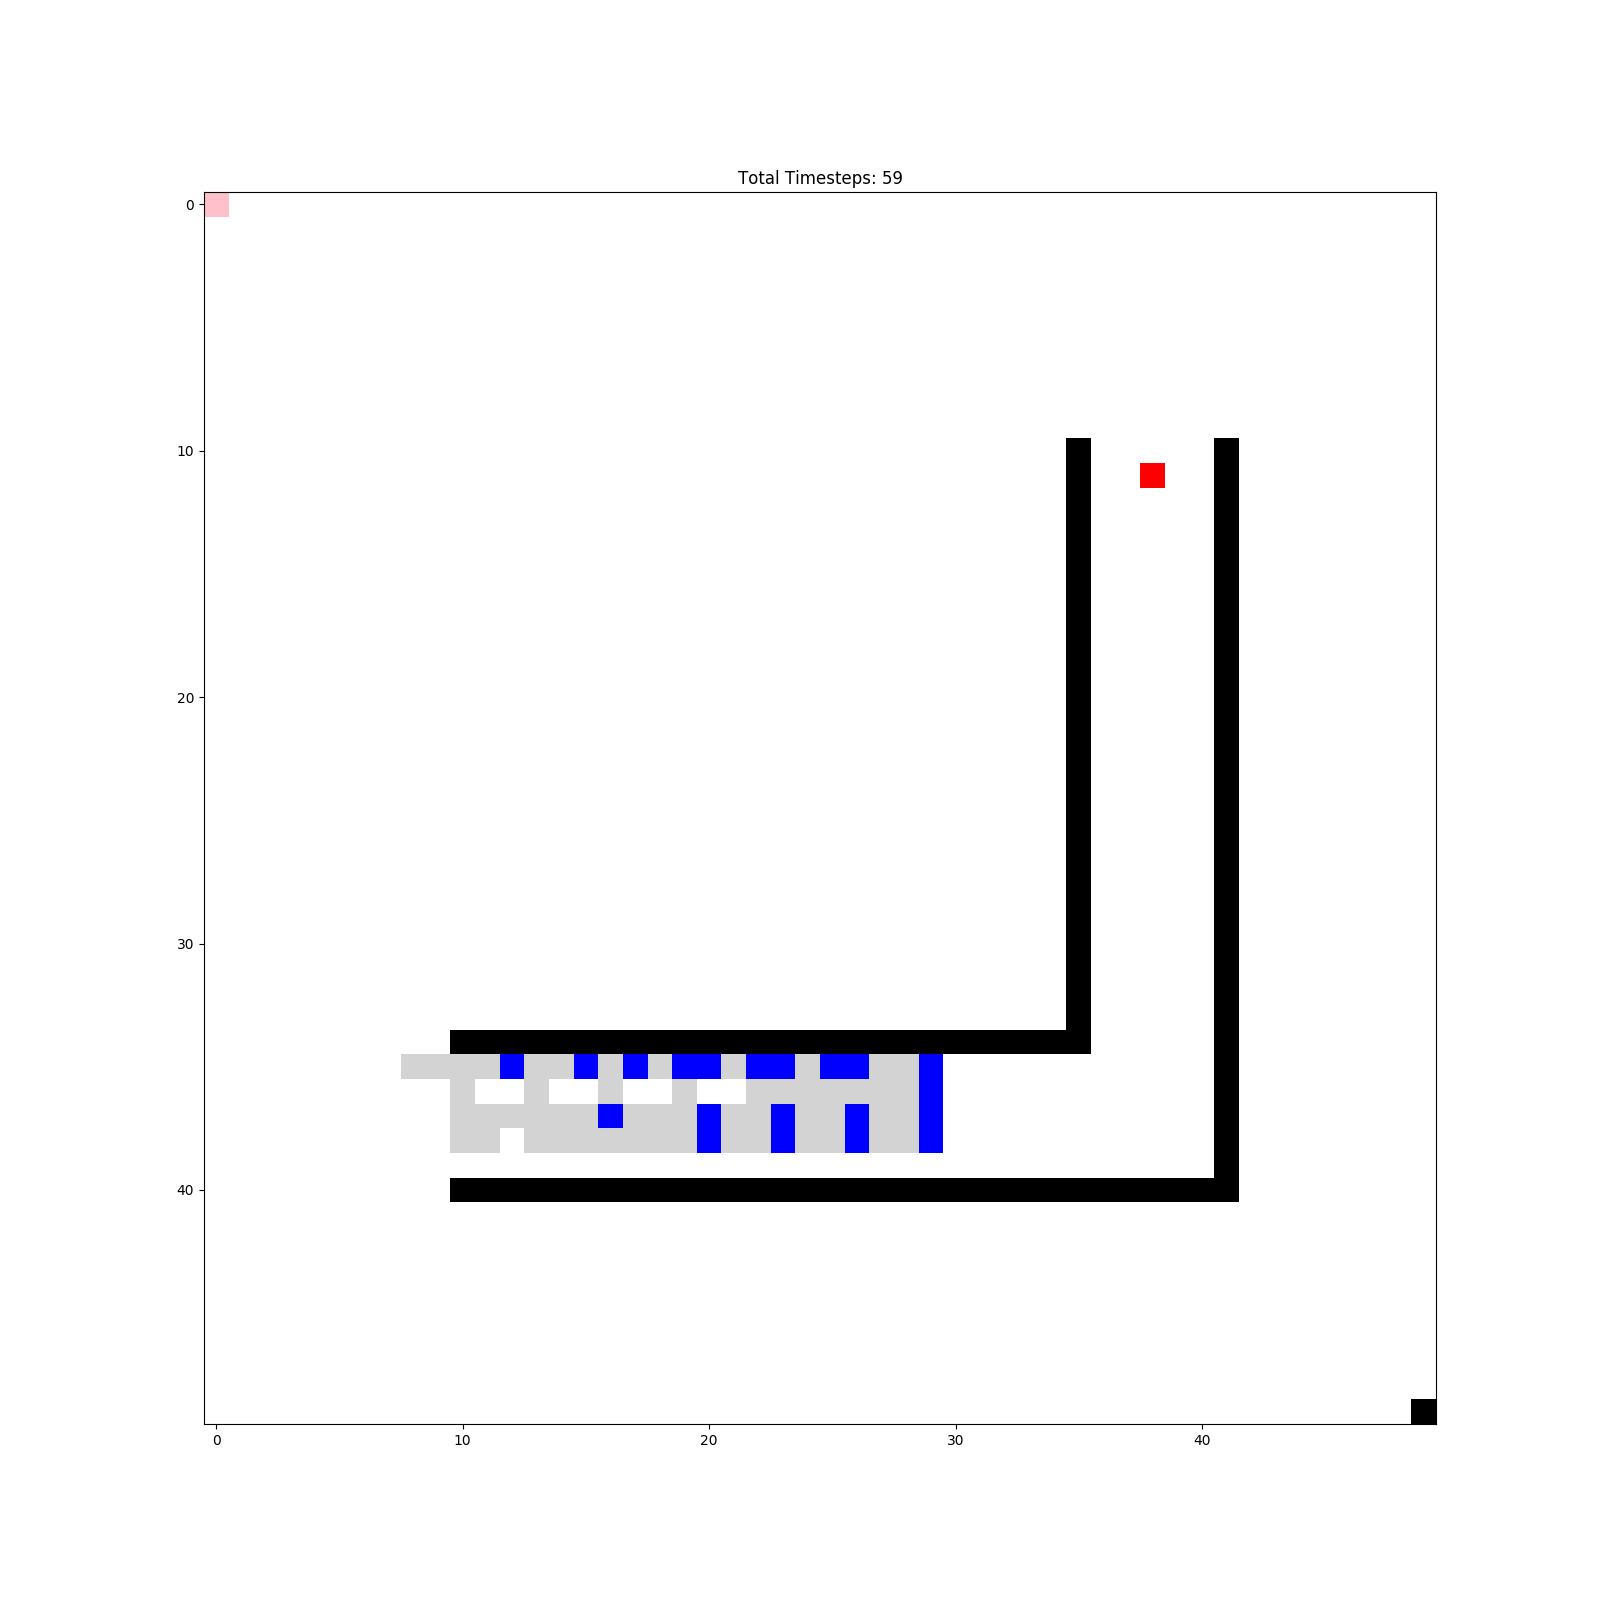
\includegraphics[width=0.6\textwidth]{pictures/Test5.png}
    \caption{Uniformly distributed pedestrians for setup of RiMEA scenario 6}
    \label{fig:test5_1}
\end{figure}
- All twenty pedestrians walked around the corner successfully without passing the walls. Figure \ref{fig:Test5_2} shows that all the pedestrians walked successfully around the corner and at figure \ref{fig:Test5_End} they all reached the red colored target. For this scenario we implemented that the pedestrians are disappearing after having reached the target, because the goal of the test is to see if the pedestrians are able to walk around the corner correctly. If we wouldn't let them disappear the pedestrians would queue around the target and block each other.
\begin{figure}[H]
    \centering
    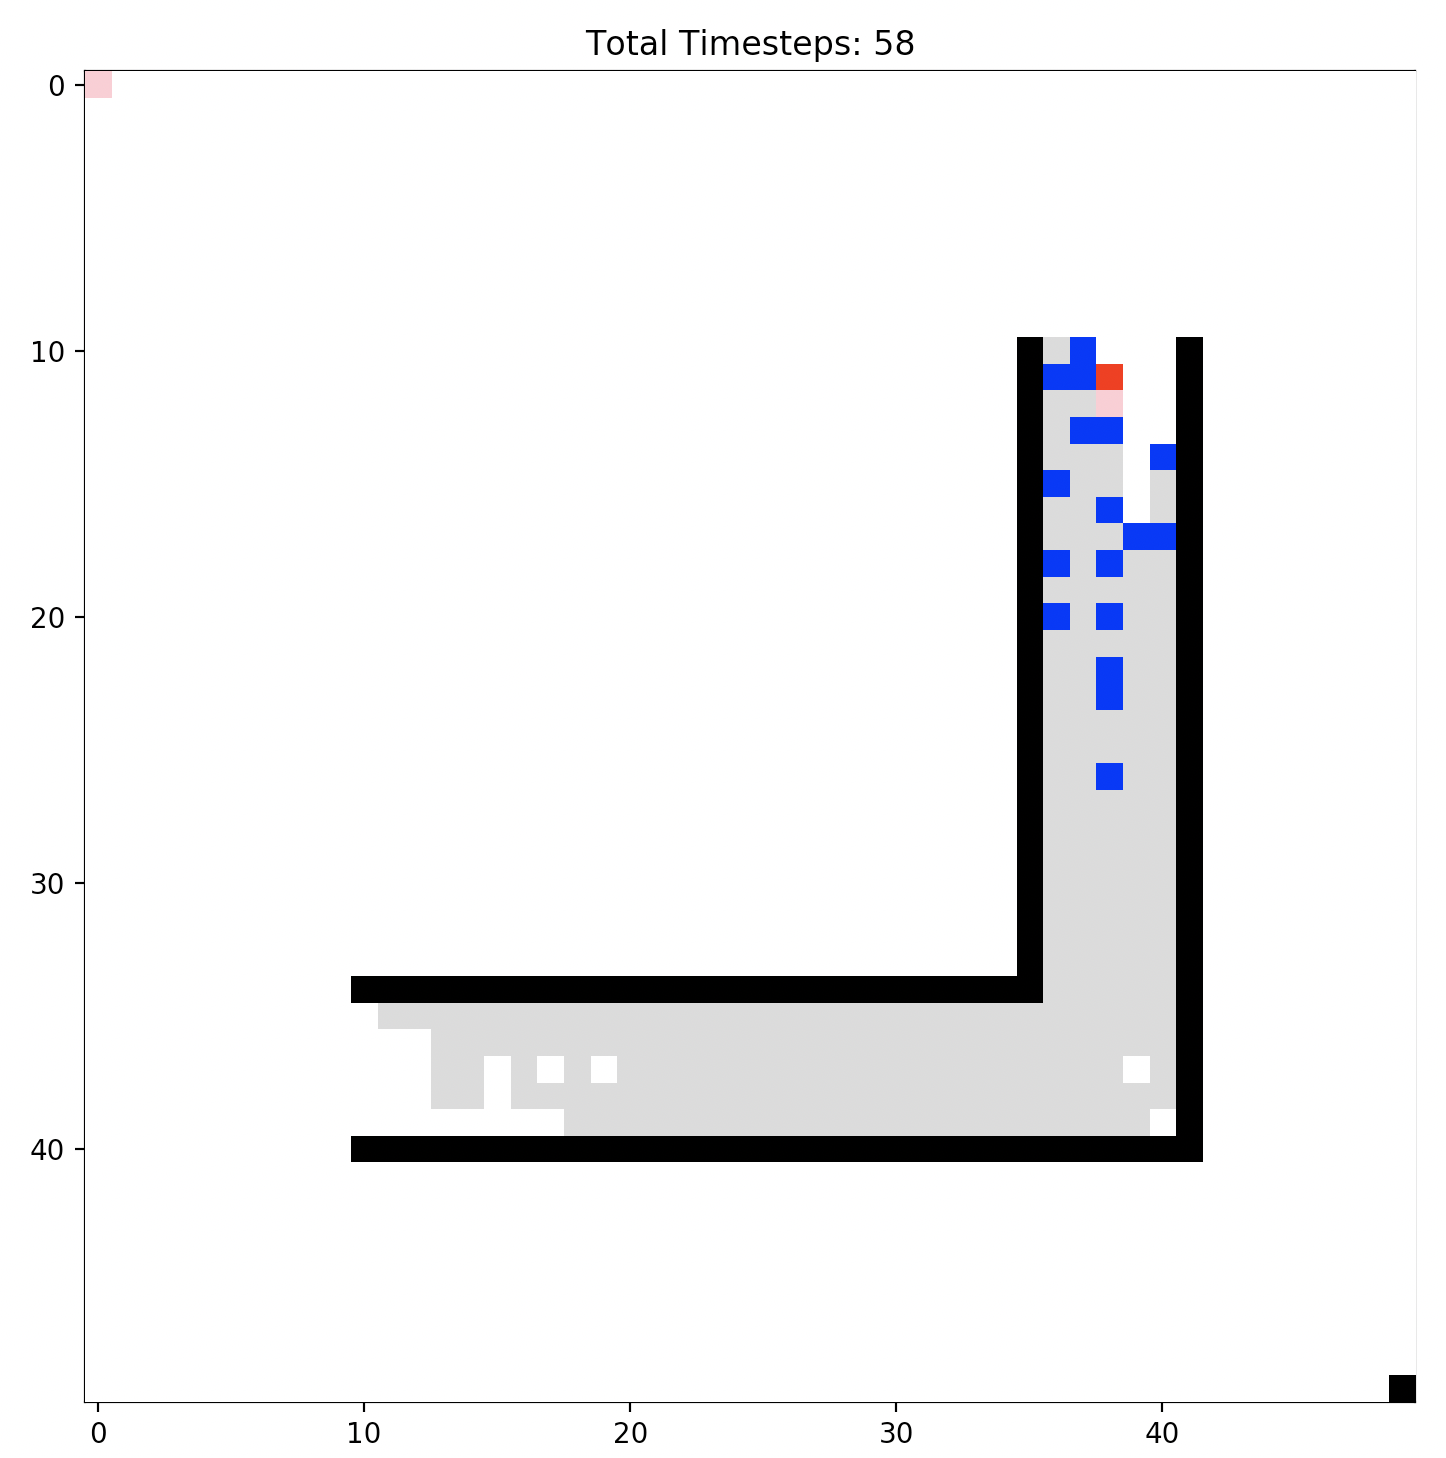
\includegraphics[width=0.5\textwidth]{pictures/Test5_meanwhile.png}
    \caption{All 20 pedestrians walked around the corner successfully}
    \label{fig:Test5_2}
\end{figure}
From Figure \ref{fig:Test5_End} can be seen that almost all cells (grey colored) were used to reach the target (red colored) around the corner.
All pedestrians walked around the corner successfully. Consequently the test is passed successfully.
- test successful - 
\begin{figure}
    \centering
    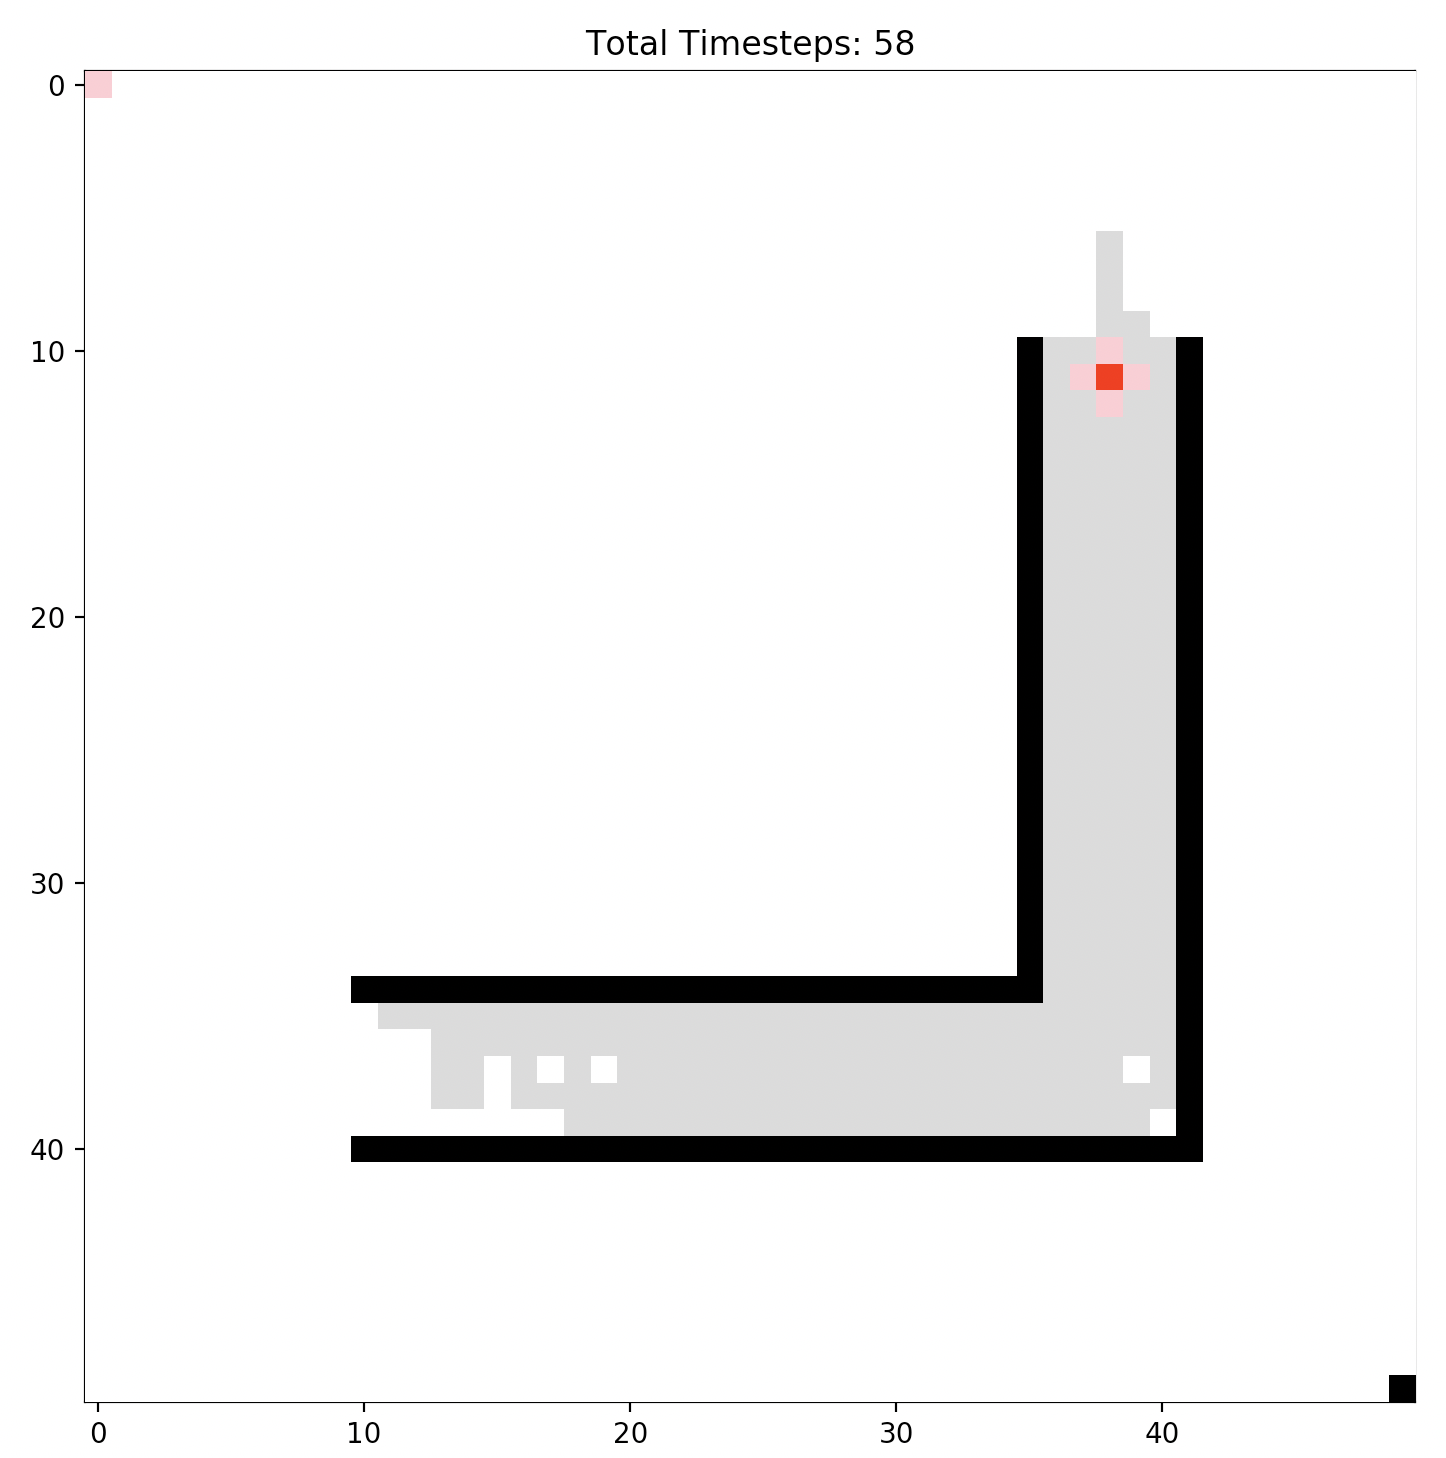
\includegraphics[width=0.5\textwidth]{pictures/Test5_End.png}
    \caption{All passengers reached the target after the corner successfully}
    \label{fig:Test5_End}
\end{figure}
\end{enumerate}
\end{task}
\end{document}